% !TeX spellcheck = en_US
% !TeX program=pdflatex
% !BIB program=biber

%%%%%%%%%%%%%%%%%%%%%%%%%%%%%%%%%%%%%%%%%%%%%%%%%%%%%%%%%%%%%%%%%%%%%%%
% NLDL 2027 submission -- adapted from the NeurIPS version (paper/paper.tex).
% Class options:
% 'fullpaper' = 5-8 page full paper; 'abstract' = 2-page extended abstract.
% 'review' (default) anonymizes the submission and adds review line numbers.
% 'final' de-anonymizes and adds the proceedings footer (needs \vol).
%%%%%%%%%%%%%%%%%%%%%%%%%%%%%%%%%%%%%%%%%%%%%%%%%%%%%%%%%%%%%%%%%%%%%%%
%\documentclass[fullpaper,final]{nldl}
\documentclass[fullpaper]{nldl}
%\documentclass[abstract]{nldl}

% TODO: replace 42 with the OpenReview submission number once available.
\paperID{42}
% Replace 'V' with the provided volume number at camera-ready time.
\vol{V}
%%%%%%%%%%%%%%%%%%%%%%%%%%%%%%%%%%%%%%%%%%%%%%%%%%%%%%%%%%%%%%%%%%%%%%%


%% Math
\usepackage{mathtools}
\usepackage{amsmath}
\usepackage{amssymb}
\usepackage{amsthm}

% Figures
\usepackage{graphicx}
% Figures live in the parent paper/ directory in this repository.
\graphicspath{{./}{../}{../n_grams_plots/}}

%% Tables
\usepackage{booktabs}
\usepackage{multirow}
\usepackage{tabularx}
\usepackage{placeins}

%% Lists
\usepackage{enumitem}

% Algorithms
\usepackage{algorithm}
\usepackage{algorithmic}
\renewcommand{\thealgorithm}{\arabic{algorithm}}

%% Diagrams
\usepackage{tikz}
\usetikzlibrary{positioning}

%% Code
\usepackage{listings}
\lstset{
  basicstyle=\small\ttfamily,
  breaklines,
}

% References
\addbibresource{references.bib}


% Links and hyperlinks
\usepackage{hyperref}
\usepackage{url}
\hypersetup{
  pdfusetitle,
  colorlinks,
  linkcolor = BrickRed,
  citecolor = NavyBlue,
  urlcolor  = Magenta!80!black,
}

%%%%%%%%%%%%%%%%%%%%%%%%%%%%%%%%
% THEOREMS
%%%%%%%%%%%%%%%%%%%%%%%%%%%%%%%%
\theoremstyle{plain}
\newtheorem{theorem}{Theorem}[section]
\newtheorem{proposition}[theorem]{Proposition}
\newtheorem{lemma}[theorem]{Lemma}
\newtheorem{corollary}[theorem]{Corollary}
\theoremstyle{definition}
\newtheorem{definition}[theorem]{Definition}
\newtheorem{assumption}[theorem]{Assumption}
\theoremstyle{remark}
\newtheorem{remark}[theorem]{Remark}

\newcommand{\cmark}{\checkmark}
\newcommand{\xmark}{\times}

% Shrink a box to the column only when it would otherwise overflow. Narrow
% tables keep their natural size instead of being blown up to \linewidth,
% which is what a bare \resizebox{\linewidth}{!} would do.
\newcommand{\fitwidth}[1]{%
  \resizebox{\ifdim\width>\linewidth\linewidth\else\width\fi}{!}{#1}}

% Graceful handling of figure assets that are not present in this checkout.
% When the real PNG is dropped next to main.tex (or in paper/), it is used
% automatically; until then a labelled placeholder keeps the document compiling.
\newcommand{\figureorplaceholder}[2]{%
  \IfFileExists{#1}{\includegraphics[width=\linewidth]{#1}}{%
    \fbox{\parbox[b][0.28\linewidth][c]{0.95\linewidth}{\centering\small
      \texttt{\detokenize{#1}} not found in this checkout.\\[2pt] #2}}}%
}


% In review mode the class replaces these with "Anonymous Full Paper Submission".
\title{Do Large Language Models Exploit Decisive Sequential Information?}
\author[1]{Anonymous Author}
\affil[1]{Anonymous Affiliation}


\begin{document}
\maketitle

\begin{abstract}
Can Large Language Models (LLMs) capture sequential structure when outcomes depend causally on order? We study this within a controlled, semantic-free sequence framework that instantiates two mechanisms: ordered-compliance (driven by strict sequential order) and global-property-compliance (driven by a global property). Theoretically, we prove that ordered-compliance inherently leaks information through frequency patterns, creating predictive shortcuts that allow models to succeed without truly capturing causal sequential structure. To isolate true order learning, we introduce a shortcut-auditing protocol that quantifies the predictive power of non-sequential features (\eg, $k$-grams, pair counts) under label noise. Empirically, encoder and recurrent models reach the theoretical optimum (measured by AUC and F1) on ordered-compliance more efficiently than fine-tuned decoder-only LLMs. Conversely, on global-property-compliance, all architectures fail under standard end-to-end training unless explicitly guided on feature relevance. Our results demonstrate that high performance on order-sensitive tasks often masks shortcut exploitation, highlighting the critical need for rigorous shortcut auditing.
\end{abstract}

\section{Introduction}
\label{sec:introduction}

Consider a clinician reviewing a patient's medical history to predict disease progression. The sequence of symptoms matters: \textit{diabetes mellitus} followed by \textit{visual disturbance} tells a different story than the same conditions appearing in reverse order for predicting \textit{myocardial infarction}~\citep{edelman2026order_specific_ehr}. Similarly, in recommendation systems, process tracing, and transaction streams, labels may depend not only on \emph{which} events occurred, but also on the \emph{order} in which they occurred. Recent electronic health record (EHR) studies use comparator cohorts that preserve event content while altering temporal structure, and show that sequence-based disease representations consistently outperform bag-of-events models by leveraging the prognostic value of directional disease progression~\citep{edelman2026order_specific_ehr,beaney2024coded_disease_representations,placido2023pancreatic_trajectories,pollington2026trajectory_review}. In recommendation, the same preferred items can reflect different user preferences when encountered in different orders~\citep{kimLostSequenceLarge2025b}.

Suppose a sequential model outperforms a bag-of-events model on clinical trajectories. Has it really learned to use order? Not necessarily. Real sequential data contain many overlapping signals: which events occur, how often, how recently, and which ones tend to appear together. A model can use any of these, or fall back on local pattern matching and lagged pair statistics, without ever recovering the causal latent trajectory rule. The difficulty is that real-world event trajectories rarely come with a known underlying mechanism, and the space of possible shortcuts is open-ended. The reason to study a controlled setting is therefore not that real-world trajectories are simple, but that they are too entangled to support mechanism attribution directly. We instantiate two complementary mechanisms, both defined over a hidden subset of letters: in \emph{ordered-compliance} (OC), these letters must appear in a secret order at a fixed lag; in \emph{global-property-compliance} (GPC), the label depends on a global property of their counts.

As LLMs and transformer-based sequential models are increasingly applied to clinical event prediction, sequential recommendation, and temporal reasoning~\citep{savcisens2024using,delphi2025transformer,li2020behrt,rasmy2021medbert,fatemiTESTTIMEBENCHMARK2025}, the relevant question is not only whether they can use order, but also whether their performance supports a claim about the mechanism they learned. Recent evidence motivates this concern: LLM-based recommenders often retain most of their performance even when item order is shuffled~\citep{kimLostSequenceLarge2025b}; clinical analyses raise concerns about statistical pattern matching rather than faithful temporal reasoning~\citep{bediFidelityMedicalReasoning2025}; and transformer predictions can often be approximated by simple $k$-gram statistics~\citep{nguyen2024understanding}.

We study this problem with a controlled letter-sequence framework in which semantic meaning and world knowledge are deliberately removed. The abstraction preserves two structural ingredients common to real-world event trajectories: only a hidden subset of letters is relevant, and labels depend on structure among those letters. A consequence of this setup, made precise in Section~\ref{sec:formulation}, is that simpler local or lagged statistics may already carry predictive signal even when the underlying mechanism is sequential; exactly the entanglement that makes shortcut auditing necessary. We prove that for non-degenerate ordered-compliance rules sampled \iid with full support, individual positions inevitably carry information about the label, formalized through \emph{single-position local purity}. The empirical question therefore shifts: rather than asking whether models use sequential structure at all, we ask how much of the label is already recoverable from local and lagged statistics, and which architectures recover them efficiently from raw sequences.

To answer this, we compare decoder-only LLMs, encoder-style transformers, and recurrent architectures against a graded series of baselines that includes contiguous $k$-grams and $\lambda$-aware pair-count classifiers. Three findings emerge: encoder-style and recurrent models reach the theoretical optimum on OC with substantially fewer parameters and less data than decoder-only LLMs; under label noise this gap widens, with decoder-only models dropping to the $k$-gram level up to 8B parameters; and on GPC all architectures remain at chance under end-to-end training, but a 64-unit MLP solves the task once subset membership is provided. Finally, a real-world clinical audit validates our core premise: even temporal dependencies can be heavily shortcut-dominated.

\paragraph{Contributions.}
\begin{itemize}[leftmargin=*,itemsep=1pt,topsep=2pt]
\item \textbf{Theory.} For OC and GPC, two label-generating mechanisms over letter sequences, we prove that they have opposite local-information structure: OC inevitably leaks single-position information, whereas balanced GPC is invisible to every proper subset of positions.
\item \textbf{Shortcut-auditing protocol.} We quantify how much outcome signal is recoverable from unordered counts, contiguous $k$-grams, lag-aware pair counts, and pair counts over all possible lags, with closed-form expressions for the theoretical optimum under label noise.
\item \textbf{Mechanism attribution.} Across decoder-only LLMs, encoder-style transformers, and recurrent models, the protocol identifies what each architecture actually learns: on OC, performance is explained by lag-aware pair-count features; on GPC, the protocol isolates subset identification as the limiting sub-task.
\item \textbf{Real-world audit.} We apply the protocol to a real clinical prediction task, demonstrating that apparent temporal sequences in real-world data can be heavily shortcut-dominated.
\end{itemize}

\section{Related work}
\label{sec:related_work}
A growing body of work in domains such as healthcare and recommendation suggests that temporal order can add predictive value beyond unordered event identity~\citep{beaney2024coded_disease_representations,placido2023pancreatic_trajectories,pollington2026trajectory_review,kimLostSequenceLarge2025b}, and transformer-based models are now routinely applied to longitudinal event histories~\citep{li2020behrt,rasmy2021medbert,savcisens2024using,delphi2025transformer}. Of particular relevance, \citet{edelman2026order_specific_ehr} study interpretable \(A\to B\to C\) clinical trajectories using comparator cohorts that preserve event content while changing temporal structure, including \(B\) without prior \(A\), reverse-order, and unordered comparisons. Such settings, together with event-log domains such as predictive process monitoring and system-log anomaly detection~\citep{teinemaa2019outcome,du2017deeplog}, motivate our question but cannot answer it directly: sequence-model gains may reflect temporal order, event semantics, co-occurrence, recency, or local event-pattern shortcuts rather than global trajectory reasoning.

Several recent benchmarks probe temporal or sequential ability~\citep{fatemiTESTTIMEBENCHMARK2025,cui2025timertemporalinstructionmodeling}, but \citet{klenitskiyDoesItLook2024} argue that many datasets marketed as sequential do not in fact require strong sequential modeling. Consistent with this, transformer behavior is often well approximated by local statistics or $k$-gram rules~\citep{nguyen2024understanding,kimLostSequenceLarge2025b,bediFidelityMedicalReasoning2025}, connecting to the broader shortcut-learning literature~\citep{mccoy2019right,geirhos2020shortcut,mirzadeh2024gsm}. At the same time, sequential models can in principle realize dependencies beyond fixed \(k\)-gram rules~\citep{olsson2022induction,guMambaLinearTimeSequence2024}.

Recent work has introduced tunable synthetic benchmarks for reasoning and sequence processing~\citep{kaiserCogniLoadSyntheticNatural2025,ramezanaliSeqBenchTunableBenchmark2025}. Our framework differs by stripping away semantics while enabling a theoretical analysis of the local-information structure of each mechanism: OC suffers unavoidable local leakage, whereas balanced GPC is invisible to every proper subset of positions. We pair the framework with a shortcut-auditing protocol that quantifies which feature families explain each model's predictions.

\section{Methods and theory}
\label{sec:formulation}
In this section, we formalize the notion of \textit{pure sequential dependence}, introduce the two experimental mechanisms of our framework, and prove theoretical properties characterizing each mechanism with respect to this property.

\paragraph{Illustrative example.}
We abstract temporal signals from domains like EHRs or recommendation into semantic-free sequences. Here, only a hidden subset of letters is predictive, and the label depends on their relative order under a rule $\kappa$ at a fixed lag $\lambda$. Our shortcut-auditing protocol tests whether models recover these latent parameters or merely exploit simpler correlates. A clinical analogy and concrete sequence walk-through are deferred to Appendix~\ref{app:illustrative}.

\subsection{Setup and notation}
\label{sec:setup}

Let $\mathcal{A}$ be an alphabet of size $\ell = |\mathcal{A}|$. Consider a hidden key subset $\mathcal{S} \subseteq \mathcal{A}$ of size $m = |\mathcal{S}|$ ($m \geq 1$) uniformly among all $m$-subsets of $\mathcal{A}$, and then sample a bijection $\kappa : \mathcal{S} \to \{1,\ldots,m\}$ uniformly among all such bijections. The realized pair $(\mathcal{S},\kappa)$ is fixed for that particular mechanism; all probabilities below are conditional on this realized pair unless stated otherwise. Symbols in $\mathcal{A}\setminus\mathcal{S}$ act as distractors and play no role in determining compliance. Let $P_0$ denote the proposal distribution over candidate sequences of length $n$: $X_t \stackrel{\mathrm{iid}}{\sim} \mathrm{Uniform}(\mathcal{A}), t=1,\ldots,n.$ This \iid uniform law is the base synthetic generation mechanism.

\begin{definition}[Ordered-Compliance Mechanism]
\label{def:compliance}
Fix a lag parameter $\lambda \geq 1$. A \emph{$\lambda$-run of key symbols}
in a sequence $X=(X_1,\ldots,X_n)$ is a tuple of positions
\[
r=(t,t+\lambda,\ldots,t+(q-1)\lambda),
\qquad q\geq 1,
\]
such that $t \geq 1$ and $t+(q-1)\lambda\leq n$, and
\[
X_{t+i\lambda}\in\mathcal{S}
\qquad
\text{for every } i=0,\ldots,q-1.
\]
The run is \emph{maximal} if it cannot be extended to the left or to the right
by another key symbol at distance $\lambda$; that is,
\[
\begin{aligned}
&t-\lambda < 1
\quad\text{or}\quad
X_{t-\lambda}\notin\mathcal{S},
\quad\text{and}\\
&t+q\lambda > n
\quad\text{or}\quad
X_{t+q\lambda}\notin\mathcal{S}.
\end{aligned}
\]
A maximal $\lambda$-run $r=(t,t+\lambda,\ldots,t+(q-1)\lambda)$ is
\emph{ordered} if $q\geq 2$ and
\[
\kappa(X_t)
\leq
\kappa(X_{t+\lambda})
\leq
\cdots
\leq
\kappa(X_{t+(q-1)\lambda}).
\]
We say that $X$ is \emph{ordered-compliant} (OC) if it contains at least one ordered
maximal $\lambda$-run.
\end{definition}

Let $Y^*=\mathbf{1}\{X \text{ is compliant}\}$, $\pi\in[0,1/2)$, and
$Y$ denote the observed label, generated from $Y^*$ according to
\begin{equation}
\label{eq:label_noise}
P(Y=1\mid Y^*=y^*)=
\begin{cases}
1-\pi, & y^*=1,\\
\pi, & y^*=0.
\end{cases}
\end{equation}

For the experiments in Sections~\ref{sec:experiments} and~\ref{sec:results}, we generate an initial oversized pool of sequences \iid from $P_0$ and compute the deterministic latent labels $Y^*$. We then stratify on $Y^*$ to create train/validation/test splits and subsamples of varying size, strictly preserving the latent prevalence reported in Table~\ref{tab:datasets}. Next, we assign the final labels $Y$ according to~\eqref{eq:label_noise}: for the deterministic setting $(\pi = 0)$, $Y = Y^*$ whereas for the noisy setting $(\pi \in (0, 1/2))$, we independently flip the labels after stratification. Note that post-stratification, the empirical distribution of the retained sequences need not be an \iid sample from $P_0$ with exactly uniform marginals. Thus, our theoretical results apply to the proposal law $P_0$, requiring only independence and full support.

\subsection{Pure sequential dependence}
\label{sec:pure_sequential_def}
We use the term \emph{pure sequential dependence} informally to denote order-sensitive tasks without local shortcuts. Since this phrase mixes order-sensitivity with distributional independence, we formalize the latter through $J$-local purity.

\begin{definition}[Local purity]
\label{def:local_purity}
Let \(X=(X_1,\ldots,X_n)\in\mathcal A^n\) and \(Y\in\{0,1\}\)
be distributed according to \(P\). For \(J\subseteq [n] = \{1, \ldots, n\}\), write
\(X_J=(X_j)_{j\in J}\), which takes values in \(\mathcal A^J\).
A task is \(J\)-locally pure under \(P\) if \(I_P(Y;X_J)=0\).
It is \emph{\(k\)-locally pure} if
\[
I_P(Y;X_J)=0
\qquad
\text{for every } J\subseteq [n] \text{ with } 1\le |J|\le k.
\]
In particular, \(1\)-local purity is equivalent to
\(I_P(Y;X_j)=0\) for every \(j\in[n]\).
For finite alphabets,
\[
\begin{aligned}
I_P(Y;X_J)
={}&
\sum_{y\in\{0,1\}}
\sum_{x_J\in\mathcal A^J}
P(Y=y,X_J=x_J)\\
&\times
\log
\frac{
P(Y=y,X_J=x_J)
}{
P(Y=y)P(X_J=x_J)
}.
\end{aligned}
\]
\end{definition}

Theorem~\ref{thm:impossibility} shows that the ordered-compliance mechanism of Definition~\ref{def:compliance} is not even 1-locally pure: there exists a single coordinate, $X_1$ under the theorem's indexing, such that $I_P(Y;X_1)>0$.

\begin{theorem}[OC Mechanism Induces Local Information]
\label{thm:impossibility}
Fix a realized pair $(\mathcal{S},\kappa)$ as in Section~\ref{sec:setup}.
Let $\lambda \ge 1$ and $n \ge \lambda+1$.
Let $X=(X_1,\ldots,X_n)$ have independent coordinates with full support on
$\mathcal{A}$, \ie\ $P(X_t=a)>0$ for all $t$ and all $a\in\mathcal{A}$.
Define
$Y^* = \mathbf{1}\{X \text{ is OC}\}$ and let $Y$ be the observed label generated from $Y^*$ according to
\eqref{eq:label_noise}. Let $\rho := P(Y^*=1)$.
If $\rho\in(0,1)$, then there exist $a,b\in\mathcal{A}$ such that $P(Y^*=1\mid X_1=a)\neq P(Y^*=1\mid X_1=b)$.
Consequently, $I(Y^*;X_1)>0$. Moreover, $P(Y=1\mid X_1=a)\neq P(Y=1\mid X_1=b)$ and therefore $I(Y;X_1)>0$.
\end{theorem}

The proof couples two sequences differing only at position~1 and shows the resulting posteriors differ; the symmetric-noise channel maps \(u=P(Y^*=1\mid X_1=a)\) to \(\pi+(1-2\pi)u\), strictly monotone for \(\pi<1/2\), so the dependence carries over to \(Y\). See Appendix~\ref{appendix:proof_impossibility}. Hence, non-degenerate OC mechanisms under independent full-support sampling are not $1$-locally pure.

\subsection{A complementary global-property-compliance mechanism}
\label{sec:parity}
While ordered-compliance inevitably leaks single-position information (Theorem~\ref{thm:impossibility}), we now introduce a complementary mechanism with the opposite information structure: global-property-compliance (GPC), in which the label requires information from the full sequence to be recovered.

\begin{definition}[Global-Property-Compliance]
\label{def:parity}
Let $\mathcal{A}$ be an alphabet of size $\ell = |\mathcal{A}|$. Fix a non-empty proper subset $K \subsetneq \mathcal{A}$.
Let $X = (X_1,\ldots,X_n)$ with $X_t \overset{\mathrm{iid}}{\sim} \mathrm{Uniform}(\mathcal{A})$.
For $k \in K$, define the count $N_k := \sum_{t=1}^n \mathbf{1}\{X_t = k\}$.
The target label is
\[
Y^* := \mathbf{1}\!\left\{
\left|\{k\in K : N_k \equiv 0 \pmod 2\}\right|
\equiv 0 \pmod 2
\right\}.
\]
Hence, $Y^* = 1$ iff an even number of key letters have an even occurrence count. Equivalently, \(Y^*\) is a fixed bit flip of the parity of $\sum_t \mathbf{1}\{X_t\in K\}$; the challenge is therefore to identify the hidden membership predicate and compute global parity over the resulting membership bits.
\end{definition}

The quantity $Y^*$ depends on the full sequence through a global parity computation over a hidden subset. Unlike the compliance family, this construction is not defined through ordered lagged chains.

\begin{theorem}[$k$-local Purity of the GPC Mechanism]
\label{thm:parity_local_purity}
Assume the setting of Definition~\ref{def:parity} with
$p := |K|/|\mathcal{A}|$. For \(J\subseteq [n] = \{1, \ldots, n\}\), write
\(X_J=(X_j)_{j\in J}\), which takes values in \(\mathcal A^J\).
Fix $n\ge 1$ and let
$J \subseteq [n]$ with $1 \le |J| < n$. Then $I(Y^*;X_J)=0$ if $p = 1/2$, and $I(Y^*;X_J)>0$ if $p \neq 1/2$. Moreover, if $p\neq 1/2$ and $J\subset \mathbb{N}$ is any fixed finite index set, interpreted as a subset of $\{1,\ldots,n\}$ for all sufficiently large~$n$, then $I(Y^*;X_J)\to 0$ as
$n\to\infty$. If the observed label $Y$ is generated from $Y^*$ via
\eqref{eq:label_noise} with $\pi<1/2$, the same qualitative statements hold with $Y$ in place of $Y^*$. In particular, when $p=1/2$, the parity task is $k$-locally pure for every $k<n$.
\end{theorem}

See Appendix~\ref{appendix:proof_parity_local_purity} for the detailed proof.

\section{Experiments}
\label{sec:experiments}

We evaluate whether different architectures recover the hidden mechanism signal beyond contiguous $k$-gram baselines, and then audit whether that signal is explained by lag-aware local features. We then apply the same shortcut-auditing logic to a real diagnosis-code prediction task in MIMIC-IV~\citep{johnson2023mimiciv}, a widely adopted public database of electronic health records, to test whether a clinically temporal task is also order-informational under a diagnosis-sequence representation. Code is available in an anonymous repository.\footnote{\url{https://anonymous.4open.science/r/anonymous_neurips_seqllm/}}

\subsection{Controlled synthetic dataset and task variants}
\label{sec:task_variants}

We instantiate the mechanisms of Section~\ref{sec:formulation} on semantic-free sequences of 20 letters over a 26-symbol alphabet. The dataset variants, summarized in Table~\ref{tab:datasets}, are designed to separate possible explanations of model success: content-frequency shortcuts, contiguous local patterns, lag-aware pair-count shortcuts, and recovery of the intended hidden mechanism.

We use $(n,\ell,m,\lambda)=(20,26,6,7)$ as a medium-difficulty anchor regime rather than a tuned optimum. With $m=6$, a sequence contains $nm/\ell \approx 4.6$ key symbols in expectation, so the hidden subset is sparse but not vanishingly rare. With $\lambda=7$, the ordered relation is non-adjacent while still providing $n-\lambda=13$ candidate lagged pairs and residue-class runs of length two or three. The resulting latent compliance rate is $\rho \approx 0.293$, giving a non-degenerate classification problem. Appendix~\ref{app:sensitivity} sweeps $m$ and $\lambda$ and shows that the qualitative conclusions are stable around this anchor.

We instantiate the \textbf{OC-Deterministic} ($\pi=0$) and \textbf{OC-Noisy} ($\pi=0.3$) variants to implement the OC mechanism (Definition~\ref{def:compliance}), extending the order-sensitive trajectory paradigm~\citep{edelman2026order_specific_ehr,placido2023pancreatic_trajectories} to a controlled synthetic setting. These variants test whether models can discover the hidden subset and lagged ordering rule, and whether their performance exceeds contiguous $k$-gram shortcuts. We also introduce the \textbf{GPC-Deterministic} variant to implement the GPC mechanism (Definition~\ref{def:parity}): its label depends on a global modular property over a hidden subset, not on temporal order, a paradigm long used as a stress test for sequence-model expressivity~\citep{hahn-2020-theoretical}. We use $|K|=6$ to match the hidden-subset size of the OC variants; the balanced $|K|=13$ regime is studied in Appendix~\ref{app:parity_vocab}.

\begin{table}[tb]
\centering
\caption{Dataset characteristics for the sequential classification task. $N_{train}$ indicates training size.}
\label{tab:datasets}
\resizebox{\linewidth}{!}{%
\begin{tabular}{lcccccc}
\toprule
Dataset & $N_{train}$ & $n$ & $\rho$ & $\lambda$ & $\pi$ & $m$ \\
\midrule
OC-Deterministic    & 400K & 20 & 0.293 & 7 & 0 & 6 \\
OC-Noisy  & 400K & 20 & 0.293 & 7 & 0.3        & 6 \\
GPC-Deterministic         & 400K & 20 & 0.499 & --& 0.0        & 6 \\
\bottomrule
\end{tabular}}
\end{table}

\subsection{Models and baselines}
\label{subsec:models}

We compare three categories of models; Table~\ref{tab:models} in Appendix~\ref{appendix:training} summarizes all configurations.

\paragraph{Pretrained LLMs (fine-tuned).} We fine-tune Llama-3.2-1B, Llama-3.1-8B and Llama-3.1-70B (the latter only on GPC-Deterministic)~\citep{touvron2023llama, grattafiori2024llama3}, Qwen3-4B-Think~\citep{bai2023qwen}, Qwen2.5-14B~\citep{qwen2.5, qwen2}, and BERT-base (110M)~\citep{devlin2019bert} and RoBERTa-large (355M)~\citep{liu2019robertarobustlyoptimizedbert} for binary classification.

\paragraph{Randomly initialized architectures.} To isolate architecture from pretrained knowledge, we train Llama-style decoders (1M), LSTM~\citep{hochreiter1997lstm}, Transformer encoder~\citep{vaswani2017attention}, and a hybrid BiLSTM-Transformer~\citep{graves2005bilstm} (RNNTransformer henceforth), each with 100K--400K parameters.

\paragraph{Traditional baselines.} XGBoost~\citep{chen2016xgboost} with two encodings: ordinal integer-mapped characters (XGBoost-basic) and, following~\citet{XGBoost_LLMs, XGBoost_LLMs_HF}, mean-pooled embeddings from Llama-3.2-1B (XGBoost-LLM). Sequences are encoded as a \texttt{Sequential events: $x_1\,\ldots\,x_n$} prompt for LLMs/BERT and as learned embeddings for randomly-initialized models (Appendix~\ref{subsec:encoding}).

\paragraph{$k$-gram and lag-aware baselines.} Three local-pattern references: (i) a contiguous $k$-gram classifier that estimates $\hat{\mathbb{P}}(Y=1\mid g) = \#(g, Y=1)/\#(g)$ and averages over the test sequence's $k$-grams (Appendix~\ref{appendix:k_gram_analysis}); (ii) a $\lambda$-aware pair-count classifier, logistic regression with $L_2$ regularization on the $26\!\times\!26$-dimensional feature $g_{ab}^{(\lambda)}$ with $\lambda$ given, which controls for whether the task can be solved by a single linear readout once the hidden offset is known; and (iii) a $\lambda$-agnostic baseline that stacks $g_{ab}^{(\lambda')}$ across all candidate offsets $\lambda' \in \{1, \ldots, n{-}1\}$ (dimension $(n{-}1)\!\times\! 676 = 12\,844$) and lets an $L_1$-regularized logistic regression or a boosted tree rediscover $\lambda$ from data. Baseline (iii) is the fair ``is the encoder's advantage about discovering $\lambda$?'' test.

\subsection{Training, evaluation, and theoretical ceiling}
\label{subsec:training}
\label{subsec:evaluation}

For the controlled synthetic tasks, all neural models are trained with AdamW~\citep{AdamW} and cross-entropy loss under early stopping. Pretrained LLMs and BERT are fine-tuned with LoRA~\citep{LoRA}, using gradient checkpointing and mixed precision for the larger models; randomly initialized models use architecture-specific learning rates and dropout; XGBoost uses regularized boosting with class weighting. We tune the decision threshold on validation to maximize F1. Experiments are run on a single NVIDIA H100 with three seeds; full hyperparameters are in Appendix~\ref{appendix:training}. Denoting by $N$ the total amount of data, we write $N_{train}$, $N_{val}$, $N_{test}$ for the Training/Validation/Test split, using a ratio of 80\%--10\%--10\%. We report AUC, F1, Precision and Recall on held-out test sets, sweeping training size from 4K to 400K.

For the synthetic mechanisms, we denote by $\mathrm{AUC}^*$ the AUC obtained by an oracle score that perfectly recovers the latent noise-free decision rule $Y^*$; see Theorem~\ref{thm:optimal_performance}. In deterministic settings ($\pi=0$), this gives $\mathrm{AUC}^*=1$. For OC-Noisy, using the latent compliance rate $\rho = P(Y^*=1)=0.293$ and noise rate $\pi=0.3$, Theorem~\ref{thm:optimal_performance} gives $\mathrm{AUC}^*=0.670$. The same theorem also reports the precision, recall, and F1 of the hard oracle classifier $\hat Y=Y^*$ evaluated against the stochastic labels: for OC-Noisy these are precision $0.700$, recall $0.491$, and F1 $0.577$. These F1-related quantities are not upper bounds under validation-threshold tuning, so we use AUC as the primary metric. We interpret $\mathrm{AUC}\approx 0.50$ as no recovery of the latent rule, $0.55<\mathrm{AUC}<\mathrm{AUC}^*$ as partial recovery, and
$\mathrm{AUC}\approx\mathrm{AUC}^*$ as full recovery up to label noise.

\subsection{Real-world audit protocol: clinical diagnosis sequences}
\label{subsec:mimic_ckd_protocol}
Moving beyond synthetic settings, motivated by~\citet{edelman2026order_specific_ehr}, we sought a real clinical task where temporal structure is plausible but model-mechanism attribution remains directly auditable. We select MIMIC-IV~\citep{johnson2024mimiciv31,johnson2023mimiciv} as our clinical testbed, given its status as a foundational machine learning benchmark and its growing adoption for evaluating LLMs in healthcare. We focus on progression from chronic kidney disease (CKD) to end-stage renal disease (ESRD), a staged renal-progression endpoint with inherently temporal clinical structure~\citep{kdigo2024ckd,sumida2017disease_trajectories_esrd}. CKD defines cohort entry, ESRD defines the future endpoint, and the model observes the pre-endpoint diagnosis history. Our question is not whether CKD progression is clinically temporal, but whether temporal order within that diagnosis history is decisive for model performance under a diagnosis-code representation. We construct a cohort of 14,813 patients (1,146 positives), mapping their specific diagnosis codes to $293$ broader Clinical Classifications Software (CCS) categories~\citep{hcup_ccs}. To prevent label leakage, we exclude patients who receive both diagnoses during the same admission. Sequences are ordered temporally across admissions and by billing order within them. We audit this task using three shortcut controls: (i) contiguous $k$-gram diagnostics, (ii) order-invariant bag-of-codes baselines (Logistic Regression, XGBoost), and (iii) sequence models evaluated on randomly shuffled patient sequences. We use AUC as the primary metric, with full cohort definitions provided in Appendix~\ref{app:mimic_ckd}.

\section{Results and discussion}
\label{sec:results}
\label{sec:discussion}

\begin{figure*}[tb]
    \centering
    \figureorplaceholder{auc_combined_main_1row.png}{Main AUC figure: test AUC vs.\ training samples for one representative model per family on OC-Deterministic, OC-Noisy, and GPC-Deterministic. Regenerate with \texttt{python -m src.analysis.plot\_main\_figure}.}
    \caption{Test AUC across three synthetic datasets. For readability, we show one representative model per family; full results across all 13 models are reported in Appendix~\ref{appendix:results}. \textbf{OC-Deterministic}: bidirectional encoders, recurrent models, and larger causal decoders (8B) reach optimality, while smaller decoders (1B) plateau at $\sim$0.85. \textbf{OC-Noisy}: bidirectional models approach the optimal bound (0.67) with modest parameter counts, while decoder-only models require substantially more parameters (14B) to reach similar performance. In \textbf{GPC-Deterministic} all models fail the task, regardless of the number of parameters (we tested up to 70B decoder-only).}
    \label{fig:comparison_AUC_all}
\end{figure*}

We evaluate all models on the three datasets of Table~\ref{tab:datasets}; Figure~\ref{fig:comparison_AUC_all} and Table~\ref{tab:results_summary} summarize the findings and Appendix~\ref{appendix:results} reports full numbers. A sanity-check task (Naive) in which all models except XGBoost achieve near-perfect AUC is reported in Appendix~\ref{app:naive}.

\paragraph{OC-Deterministic: bidirectional and recurrent models learn the offset efficiently.}
When compliance requires detecting a lag-7 ordered key run, pretrained bidirectional encoders (BERT, RoBERTa) and small randomly initialized sequential models (Transformer, LSTM, RNNTransformer; 100K--400K parameters) reach AUC \(\ge 0.997\). Decoder-only Llama-3.2-1B plateaus at AUC \(\approx 0.85\), close to the contiguous 2-gram baseline of 0.82, while Llama-3.1-8B reaches AUC $=0.995$. XGBoost on frozen Llama-3.2-1B mean-pooled embeddings also fails; this likely reflects a mismatch between pretrained representations and our synthetic letter task rather than a property of the embedding architecture per se. The mechanism-identification audit of Section~\ref{sec:mechanism_id} shows that a 676-dimensional logistic regression on the \(\lambda\)-aware pair feature \(g_{ab}^{(\lambda=7)}\) also reaches AUC $=0.997$, and that a \(\lambda\)-agnostic 12,844-dimensional logistic regression recovers \(\lambda=7\) on its own. We therefore read the encoder--decoder gap on this task as an efficiency gap in discovering the right lagged-pair feature from raw-token supervision, rather than as evidence for global sequence integration.

\paragraph{OC-Noisy: scale unlocks autoregressive models.}
At $\pi=0.3$ the theoretical upper bound is $\mathrm{AUC}^*=0.67$. Our custom Transformer and RNNTransformer reach this ceiling (AUC $=0.671$), BERT reaches AUC $=0.669$, and LSTM reaches AUC$=0.665$. Smaller decoder-only models (Llama-3.2-1B, 8B) plateau near AUC$=0.587$, close to the contiguous 2-gram baseline ($=0.585$), but at sufficient scale Qwen-14B also approaches the ceiling. The mechanism-identification ladder again matches the ceiling with a linear model when $\lambda$ is given ($L_2$ logistic regression on $g_{ab}^{(\lambda=7)}$, AUC $=0.671$) and with a boosted tree when $\lambda$ is not given ($\lambda$-agnostic XGBoost on stacked all-offset pair counts, AUC $=0.667$). The $\lambda$-agnostic linear baseline underperforms the ceiling (AUC $=0.632$): under label noise the right $\lambda$-block is not separable by a linear sparsity pattern and the top-weight lag on $L_1$ logistic regression drifts to $\lambda=19$ (Appendix~\ref{appendix:mechanism_id}). Decoder-only models can reach the ceiling at sufficient scale in our tested regime, but require substantially more parameters than encoders to match what a boosted tree does with hand-crafted pair features.

\paragraph{GPC-Deterministic: a hidden-subset identification failure, not a modular-arithmetic failure.}
Every tested model is at chance (AUC $\approx 0.50$) on hidden-subset parity, including 70B-parameter LLMs, bidirectional transformers, and recurrent networks; the $k$-gram baselines also fail, consistent with \citet{countingLLMs}. This holds both in the main $|K|=6$ regime and, for the core architectures, in the exactly balanced $|K|=13$ regime (Appendix~\ref{appendix:mechanism_id}). A decomposition (Appendix~\ref{appendix:parity_decomp}) localizes the failure to joint hidden-subset identification and modular arithmetic under end-to-end supervision, rather than to modular arithmetic itself: a 64-unit MLP fed the per-position membership bits $b_t = \mathbf{1}\{X_t \in K\}$ (a 20-dim binary input that does not name the key letters) reaches AUC $=0.997$ in under a minute, and AUC $=1.000$ when fed the 6-dim per-key parity vector. Binary-vocabulary parity and induction-head circuits succeed on related tasks~\citep{olsson2022induction}; we reproduce one such protocol and locate our regime on the non-learnable side of a length-driven phase boundary (Appendix~\ref{appendix:parity_reference}). The negative result is therefore about end-to-end supervised learning of hidden-subset identification, not a general claim on parity learnability. Few-shot in-context evaluation of Llama-3.2-1B, Llama-3.1-8B, and Qwen2.5-14B fails on both OC variants and on GPC, indicating the main fine-tuning results are not an artifact of access mode (Appendix~\ref{appendix:fewshot}).

\begin{table}[tb]
\centering
\caption{Summary of model performance across datasets, using criteria from Section~\ref{subsec:evaluation}. $\cmark$: full recovery (AUC $\approx$ AUC$^*$); {\raise.17ex\hbox{$\scriptstyle\sim$}}: partial recovery ($0.55 <$ AUC $<$ AUC$^*$); $\xmark$: no learning (AUC $\approx 0.50$). $\bigstar$: most data-efficient models to reach the optimum. $-$: not tested on that dataset. All evaluations based on 100\% training data.}
\label{tab:results_summary}
\small
\begin{tabular}{@{}lccc@{}}
\toprule
Model & OC-Det. & OC-Noisy & GPC-Det. \\
\midrule
$k$-gram baseline & {\raise.17ex\hbox{$\scriptstyle\sim$}} & {\raise.17ex\hbox{$\scriptstyle\sim$}} & $\xmark$ \\
XGBoost & {\raise.17ex\hbox{$\scriptstyle\sim$}} & $\xmark$ & $\xmark$ \\
BERT & $\bigstar$ & $\bigstar$ & $\xmark$ \\
RoBERTa & $\cmark$ & $\cmark$ & $\xmark$ \\
Llama-3.2-1B & {\raise.17ex\hbox{$\scriptstyle\sim$}} & {\raise.17ex\hbox{$\scriptstyle\sim$}} & $\xmark$ \\
Qwen3-4B-Think & {\raise.17ex\hbox{$\scriptstyle\sim$}} & {\raise.17ex\hbox{$\scriptstyle\sim$}} & $\xmark$ \\
Llama-3.1-8B & $\cmark$ & {\raise.17ex\hbox{$\scriptstyle\sim$}} & $\xmark$ \\
Qwen2.5-14B & $-$& $\cmark$ & $-$ \\
Llama-3.1-70B  & $-$ & $-$ & $\xmark$ \\
LSTM & $\cmark$  & $\cmark$ & $\xmark$ \\
Transformer & $\bigstar$ & $\bigstar$ & $\xmark$ \\
RNNTransformer$^{*}$ & $\cmark$ & $\cmark$ & $\xmark$ \\
\bottomrule
\multicolumn{4}{@{}l@{}}{\footnotesize $^{*}$We call RNNTransformer a BiLSTM-Transformer.}
\end{tabular}
\end{table}

\subsection{Mechanism-identification audit and sensitivity sweep}
\label{sec:mechanism_id}

To explain the drivers of model performance, we evaluate a hierarchy of seven feature sets across three simple classifiers (Appendix~\ref{appendix:mechanism_id}). On both OC variants, a logistic regression trained solely on lag-aware aggregated pair counts perfectly matches the encoder ceiling, whereas simple content counts fall short (AUC $0.82$ for deterministic, $0.58$ for noisy). We contextualize this linear performance through two controls. First, a leave-one-rule-out experiment reveals that the linear model learns rule-specific weights rather than a transferable algorithm (within-rule AUC $1.00$ \vs across-rule AUC $0.50$; Appendix~\ref{appendix:heldout}). Second, even after matching on key-letter counts, lag-aware features retain a non-trivial predictive signal (within-group AUC $0.65$ \vs chance $0.50$ on OC-Noisy). Internally, attention analysis confirms that while BERT suppresses non-key positions, it does not preferentially attend to lag-connected key pairs (Appendix~\ref{appendix:attention}). Finally, a sensitivity sweep over $m$ and $\lambda$ (Appendix~\ref{app:sensitivity}) preserves the same qualitative pattern: BERT and LSTM operate near the oracle ceiling, while Llama-3.2-1B remains consistently less efficient.

\subsection{A length-based curriculum partially recovers the GPC mechanism}
\label{sec:curriculum}
\citet{hahn-2020-theoretical} identifies length-dependent difficulties for transformer parity learning (the key ingredient of our GPC mechanism), consistent with what we observe: small encoders learn parity at $n=10$ but collapse to chance at $n=20$ (Appendix~\ref{appendix:parity_reference}). We exploit this gap with a two-stage curriculum: train from scratch on $n=10$, then warm-start on $n=20$ with positional embeddings transferred where applicable. This recovers global-property-compliance for an LSTM and for a small randomly initialized Transformer, but not for pretrained BERT or Llama under our tested recipes (Appendix~\ref{app:parity_curriculum}). The bottleneck for shallow random-init architectures is therefore addressable by training-paradigm interventions, while pretrained models require additional study.

\subsection{Real-world audit: limited gains can reflect non-decisive sequential information}
\label{sec:mimic_ckd_results}
Our empirical results demonstrate that for CKD$\to$ESRD progression, the prediction task becomes heavily shortcut-dominated under a diagnosis-code representation. Unigrams alone capture most of the predictive signal (AUC $0.823 \pm 0.015$), outperforming contiguous 2-grams ($0.801 \pm 0.016$). Order-invariant baselines are similarly strong, with Logistic Regression and XGBoost reaching AUCs of 0.809 and 0.803, respectively. A Transformer achieves the peak ordered AUC (0.860), but most of this gain remains after randomly shuffling each patient's sequence (AUC 0.844), while BiLSTM and BERT show no ordered-versus-shuffled gain. In this representation, the task can be solved by exploiting diagnosis identity, frequency, and co-occurrence: learning \emph{what} diagnoses occur is largely sufficient, so learning \emph{when} they occur is not decisive for performance. Full results in Appendix~\ref{app:mimic_ckd}.

\section{Discussion and limitations}
\label{sec:limitations}
This work introduced a semantic-free diagnostic framework to test whether sequence models recover the intended latent mechanism or exploit simpler predictive shortcuts. The two mechanisms expose complementary regimes. In the OC mechanism, models can perform well by discovering lag-aware pair-count features; indeed, these features match the empirical ceiling reached by the best encoders. Thus, strong OC performance should be interpreted as efficient recovery of the relevant lagged statistic, not as evidence of global sequence integration. In the GPC mechanism, all models fail under standard end-to-end training, while the task becomes solvable once hidden membership information is provided. This localizes the difficulty to joint hidden-subset identification and global aggregation.

From the theoretical perspective, Theorem~\ref{thm:impossibility} is specific to the OC mechanism and does not extend to arbitrary order-sensitive labels. For example, if $\mathcal{A}=\{0,1,2,3,4\}$, $X_t \overset{\mathrm{iid}}{\sim} \mathrm{Uniform}(\mathcal{A})$, and $Y=\mathbf{1}\{(X_2+2X_3)\bmod 5 \in \{0,1\}\}$, then $I(Y;X_t)=0$ for every $t$, although $Y$ depends on the ordered pair $(X_2,X_3)$. The theorem also guarantees only the existence of single-position leakage, but does not provide a theoretical lower bound on its magnitude. Theorem~\ref{thm:parity_local_purity} should be read as a bounded-local result.

The synthetic setting is intentionally narrow. It targets two capabilities: recovering a hidden positional offset from raw tokens, and jointly identifying a hidden subset while applying a global modular rule. It is not a general benchmark for long-range sequential learning. Empirically, we focus on one main regime per task, with sensitivity sweeps and ablations in the appendix; most models are tested up to 14B parameters, with the 70B model evaluated only on the GPC mechanism. The theoretical claims also rely on independent full-support sampling and should not be read as impossibility results for arbitrary real-world sequence distributions, transformers, or parity-like tasks in general.

Finally, our MIMIC-IV audit is limited to a single clinical case study. However, as recent work highlights~\citep{edelman2026order_specific_ehr}, while true temporal dependencies certainly exist in clinical trajectories, they are neither ubiquitous nor trivial to isolate. Therefore, judging a sequence model's architectural adequacy based solely on its raw performance on real-world sequential tasks requires extreme caution. Although our case study is not an exhaustive benchmark, it efficiently demonstrates a broader fundamental principle: apparent sequentiality in real data does not imply an absence of predictive shortcuts.

\printbibliography

\appendix

\paragraph{Appendix roadmap.}
Appendices A--F provide task examples, proofs, and reproducibility details. Appendix G reports full model results. Appendix H tests robustness of the compliance findings across subset size and lag. Appendix I contains the mechanism-identification audits and additional parity controls used to rule out alternative explanations. Appendix J provides an exploratory attention inspection; we do not use it as primary evidence for mechanism attribution.

\begin{table}[tb]
\centering
\caption{Purpose of appendix analyses.}
\resizebox{\linewidth}{!}{%
\begin{tabular}{ll}
\toprule
Appendix & Purpose \\
\midrule
\ref{app:illustrative} & Real-world motivation \\
\ref{app:naive} & Naive Sanity Check \\
\ref{appendix:Figures} & Ordering Mechanism Example \\
\ref{appendix:k_gram_analysis} & Contiguous k-gram shortcut analysis \\
\ref{appendix:proof_theorems} & Proofs of local leakage and parity purity \\
\ref{appendix:training} & Reproducibility and model configurations \\
\ref{appendix:results} & Full numerical results \\
\ref{app:sensitivity} & Sensitivity to hidden-subset size and lag \\
\ref{appendix:ladder}--\ref{appendix:parity_decomp} & Mechanism-identification audit \\
\ref{appendix:parity_reference}--\ref{app:parity_length} & Parity robustness checks \\
\ref{appendix:fewshot} & In-context access-mode control \\
\ref{app:parity_curriculum} & Curriculum control for parity learnability \\
\ref{appendix:attention} & Exploratory attention inspection, not primary evidence \\
\bottomrule
\end{tabular}}
\end{table}

\section{Real-world trajectory motivation and synthetic abstraction}
\label{app:illustrative}

Consider adverse-outcome prediction from longitudinal EHRs. 
\citet{edelman2026order_specific_ehr} study order-specific trajectories of the form \(A\to B\to C\): two upstream events \(A\) and \(B\) define an ordered exposure, and \(C\) is a downstream adverse outcome. Their comparator design asks whether the ordered exposure \(A\to B\) changes risk relative to cohorts that preserve part of the same event content while altering temporal structure, including \(B\) with no prior \(A\), the reverse ordering \(B\to A\), and an unordered \(AB\) cohort. One validated example is diabetes mellitus \(\to\) visual disturbance for downstream myocardial infarction; at the five-year horizon, the ordered trajectory has elevated risk relative to both the primary comparator and the reverse-order comparator. We use this only as a motivating analogy: the association is prognostic rather than causal, and our benchmark does not model clinical outcomes, censoring, observation processes, or risk calibration. In particular, the clinical \(C\) is a future outcome, whereas \(Y^*\) in our compliance task is a synthetic label indicating whether a hidden ordered motif is present.

Our synthetic tasks abstract only the mechanism-attribution problem exposed by such studies. In real EHRs, a model's success may come from event identity, disease semantics, code frequency, recency, care-utilization patterns, or local co-occurrence rather than from the intended temporal rule. We therefore replace event types by letters and remove semantic content: for exposition, diabetes mellitus can be denoted \texttt{D} and visual disturbance \texttt{V}, but these mnemonic choices are not used in the benchmark. In the experiments, the relevant subset and the ordering rule \(\kappa\) are hidden and randomized, so a model cannot exploit medical meaning, alphabetical order, or pre-existing associations.

As a toy walk-through, let a patient history be represented by
\[
X=\texttt{BXDQAVZHELNPTKDWSRAJ},
\]
with length \(n=20\). Suppose the hidden key subset is \(S=\{\texttt{D},\texttt{V}\}\), with \(\kappa(\texttt{D})<\kappa(\texttt{V})\), and let \(\lambda=3\). Then positions \(3\) and \(6\) form a lag-\(\lambda\) ordered key pair, \(\texttt{D}\to\texttt{V}\), so the sequence is compliant. The lag \(\lambda\) is only a discrete abstraction of temporal spacing; it is not intended to represent a clinical time interval such as days or years. A rule-based solution would require recovering which letters matter, their ordering, and the relevant lag. The purpose of our audit is to determine whether neural models recover this hidden structure from raw tokens or whether their performance is already explained by simpler feature families such as unordered counts, contiguous \(k\)-grams, or lag-aware pair counts.


\section{Degenerate local sanity check: Naive}
\label{app:naive}

We include \textbf{Naive} only as a pipeline sanity check, not as a core benchmark.
Here $m=\ell$, $\lambda=1$, and $\kappa$ is the natural alphabetical order, so
$Y^*=1$ iff the entire sequence is non-decreasing. This construction makes
the label locally detectable: descending adjacent bigrams occur only in negatives, and
a contiguous 2-gram classifier reaches AUC $\approx 0.999$. Consistent with this, all neural sequential models reach
near-perfect AUC with $\ge 40$K training examples, while XGBoost without explicit
adjacent-pair features does not (Table~\ref{tab:results_full}). We therefore use Naive
only to verify the training and evaluation pipeline, and exclude it from the main
benchmark.

\section{Compliance Mechanisms}
\begin{figure*}[tb]
\centering
\resizebox{\textwidth}{!}{%
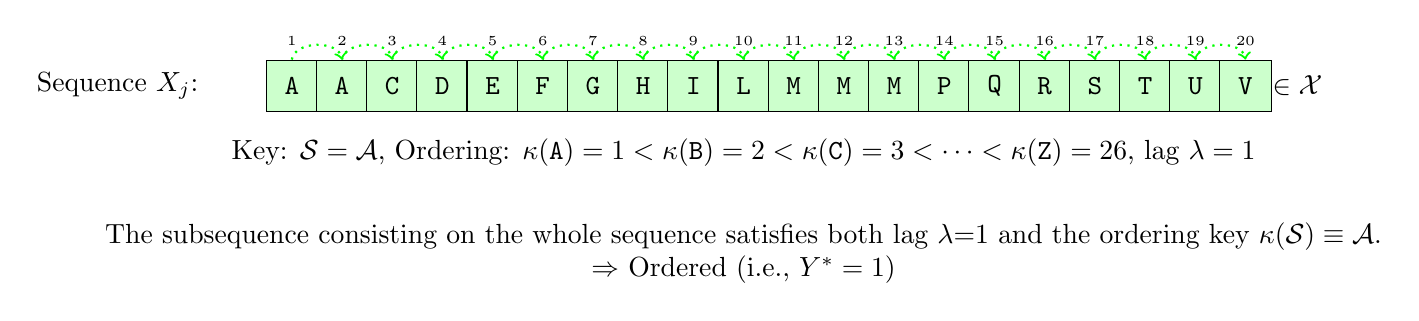
\begin{tikzpicture}[scale=0.85]
% Full sequence with key letters highlighted
\foreach \i/\letter in {1/\texttt{A},2/\texttt{A},3/\texttt{C},4/\texttt{D},5/\texttt{E},6/\texttt{F},7/\texttt{G},8/\texttt{H},9/\texttt{I},10/\texttt{L},11/\texttt{M},12/\texttt{M},13/\texttt{M},14/\texttt{P},15/\texttt{Q},16/\texttt{R},17/\texttt{S},18/\texttt{T},19/\texttt{U},20/\texttt{V}} {
    \node[draw,minimum size=0.65cm,text=black, fill=green!20] (n\i) at (\i*0.75,0) {\letter};
}
\node[anchor=east] at (-0.5,0) {Sequence $X_j$:};
\node[right=12cm of n1] {$\in \mathcal{X}$};

% Position numbers above key letters
\node[above=0.05cm of n1,black,font=\tiny] {1};
\node[above=0.05cm of n2,black,font=\tiny] {2};
\node[above=0.05cm of n3,black,font=\tiny] {3};
\node[above=0.05cm of n4,black,font=\tiny] {4};
\node[above=0.05cm of n5,black,font=\tiny] {5};
\node[above=0.05cm of n6,black,font=\tiny] {6};
\node[above=0.05cm of n7,black,font=\tiny] {7};
\node[above=0.05cm of n8,black,font=\tiny] {8};
\node[above=0.05cm of n9,black,font=\tiny] {9};
\node[above=0.05cm of n10,black,font=\tiny] {10};
\node[above=0.05cm of n11,black,font=\tiny] {11};
\node[above=0.05cm of n12,black,font=\tiny] {12};
\node[above=0.05cm of n13,black,font=\tiny] {13};
\node[above=0.05cm of n14,black,font=\tiny] {14};
\node[above=0.05cm of n15,black,font=\tiny] {15};
\node[above=0.05cm of n16,black,font=\tiny] {16};
\node[above=0.05cm of n17,black,font=\tiny] {17};
\node[above=0.05cm of n18,black,font=\tiny] {18};
\node[above=0.05cm of n19,black,font=\tiny] {19};
\node[above=0.05cm of n20,black,font=\tiny] {20};

% Key information - moved down more
\node at (7.5,-1) {Key: $\mathcal{S} = \mathcal{A}$, Ordering: $\kappa(\texttt{A})=1 < \kappa(\texttt{B})=2 < \kappa(\texttt{C})=3 < \cdots < \kappa(\texttt{Z})=26$, lag $\lambda=1$};

% Arrows showing different paths - all starting lower and with better spacing

\draw[->,thick,green,dotted] (n1.north) to[out=80,in=100] (n2.north);
\draw[->,thick,green,dotted] (n2.north) to[out=80,in=100] (n3.north);
\draw[->,thick,green,dotted] (n3.north) to[out=80,in=100] (n4.north);
\draw[->,thick,green,dotted] (n4.north) to[out=80,in=100] (n5.north);
\draw[->,thick,green,dotted] (n5.north) to[out=80,in=100] (n6.north);
\draw[->,thick,green,dotted] (n6.north) to[out=80,in=100] (n7.north);
\draw[->,thick,green,dotted] (n7.north) to[out=80,in=100] (n8.north);
\draw[->,thick,green,dotted] (n8.north) to[out=80,in=100] (n9.north);
\draw[->,thick,green,dotted] (n9.north) to[out=80,in=100] (n10.north);
\draw[->,thick,green,dotted] (n10.north) to[out=80,in=100] (n11.north);
\draw[->,thick,green,dotted] (n11.north) to[out=80,in=100] (n12.north);
\draw[->,thick,green,dotted] (n12.north) to[out=80,in=100] (n13.north);
\draw[->,thick,green,dotted] (n13.north) to[out=80,in=100] (n14.north);
\draw[->,thick,green,dotted] (n14.north) to[out=80,in=100] (n15.north);
\draw[->,thick,green,dotted] (n15.north) to[out=80,in=100] (n16.north);
\draw[->,thick,green,dotted] (n16.north) to[out=80,in=100] (n17.north);
\draw[->,thick,green,dotted] (n17.north) to[out=80,in=100] (n18.north);
\draw[->,thick,green,dotted] (n18.north) to[out=80,in=100] (n19.north);
\draw[->,thick,green,dotted] (n19.north) to[out=80,in=100] (n20.north);

% Results - moved down even more
\node[align=center] at (7.5,-2.5) {The subsequence consisting on the whole sequence satisfies both lag $\lambda$=1 and the ordering key $\kappa(\mathcal{S}) \equiv \mathcal{A}$.\\
$\Rightarrow$ Ordered (i.e., $Y^{*}=1$)};
\end{tikzpicture}%
}
\caption{Sequence classification example in the \textbf{Naive} sanity check. Key letters $\mathcal{S} = \mathcal{A}$ (i.e., all letters). Arrows show gaps between key letters.
In green letters (and gaps) that do have lag-connections with other key letters and that satisfy the ordering $\kappa(\mathcal{S}) \equiv \mathcal{A}$. Note: in this example $n=20$, $m=26$.}
\label{fig:naive_example}
\end{figure*}

\label{appendix:Figures}
\begin{figure*}[tb]
\centering
\resizebox{\textwidth}{!}{%
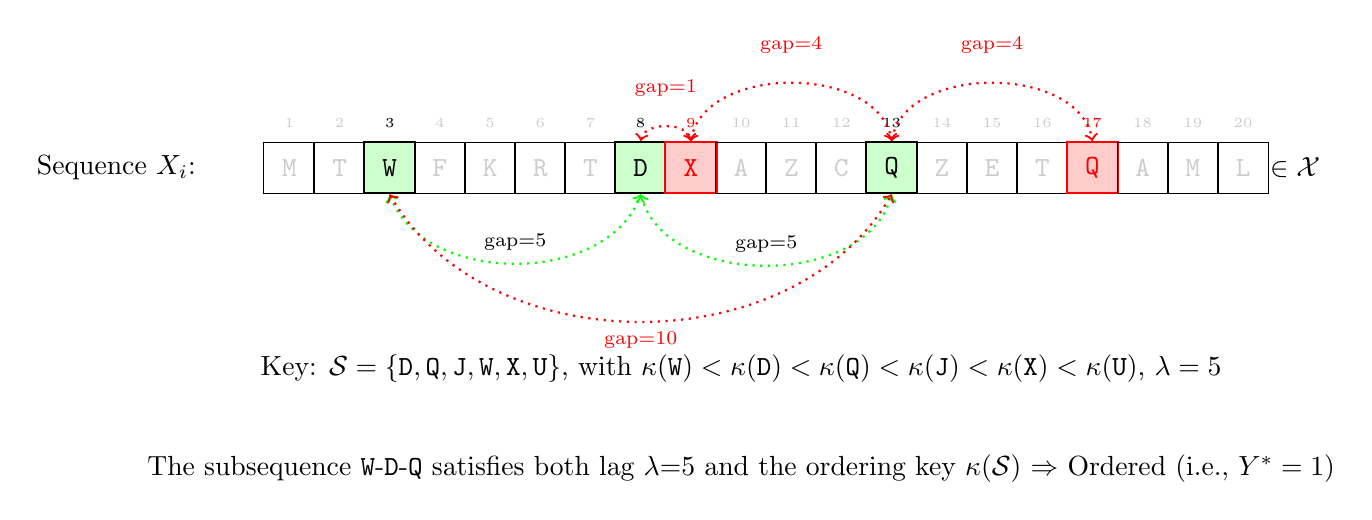
\begin{tikzpicture}[scale=0.85, baseline=(current bounding box.center)]
% Full sequence with key letters highlighted
\foreach \i/\letter in {1/\texttt{M},2/\texttt{T},3/\texttt{W},4/\texttt{F},5/\texttt{K},6/\texttt{R},7/\texttt{T},8/\texttt{D},9/\texttt{X},10/\texttt{A},11/\texttt{Z},12/\texttt{C},13/\texttt{Q},14/\texttt{Z},15/\texttt{E},16/\texttt{T},17/\texttt{Q},18/\texttt{A},19/\texttt{M},20/\texttt{L}} {
    % Check prima se è posizione 9 (rosso)
    \ifnum\i=9
        \node[draw,thick,red,minimum size=0.65cm,fill=red!20] (n\i) at (\i*0.75,0) {\textbf{\letter}};

    \else
        \ifnum\i=17
            \node[draw,thick,red,minimum size=0.65cm,fill=red!20] (n\i) at (\i*0.75,0) {\textbf{\letter}};
        \else
            % Altrimenti check se è 3, 8 o 13 (arancione)
            \pgfmathparse{\i==3 || \i==8 || \i==13 ? 1 : 0}
            \ifnum\pgfmathresult=1
                \node[draw,thick,black,minimum size=0.65cm,fill=green!20] (n\i) at (\i*0.75,0) {\textbf{\letter}};
            \else
                % Altrimenti grigio
                \node[draw,minimum size=0.65cm,text=gray!40] (n\i) at (\i*0.75,0) {\letter};
            \fi
        \fi
    \fi
}
\node[anchor=east] at (-0.5,0) {Sequence $X_i$:};
\node[right=12cm of n1] {$\in \mathcal{X}$};

% Position numbers above key letters
\node[above=0.05cm of n1,gray!40,font=\tiny] {1};
\node[above=0.05cm of n2,gray!40,font=\tiny] {2};
\node[above=0.05cm of n3,black,font=\tiny] {3};
\node[above=0.05cm of n4,gray!40,font=\tiny] {4};
\node[above=0.05cm of n5,gray!40,font=\tiny] {5};
\node[above=0.05cm of n6,gray!40,font=\tiny] {6};
\node[above=0.05cm of n7,gray!40,font=\tiny] {7};
\node[above=0.05cm of n8,black,font=\tiny] {8};
\node[above=0.05cm of n9,red,font=\tiny] {9};
\node[above=0.05cm of n10,gray!40,font=\tiny] {10};
\node[above=0.05cm of n11,gray!40,font=\tiny] {11};
\node[above=0.05cm of n12,gray!40,font=\tiny] {12};
\node[above=0.05cm of n13,black,font=\tiny] {13};
\node[above=0.05cm of n14,gray!40,font=\tiny] {14};
\node[above=0.05cm of n15,gray!40,font=\tiny] {15};
\node[above=0.05cm of n16,gray!40,font=\tiny] {16};
\node[above=0.05cm of n17,red,font=\tiny] {17};
\node[above=0.05cm of n18,gray!40,font=\tiny] {18};
\node[above=0.05cm of n19,gray!40,font=\tiny] {19};
\node[above=0.05cm of n20,gray!40,font=\tiny] {20};

% Key information - moved down more
\node at (7.5,-3) {Key: $\mathcal{S} = \{\texttt{D}, \texttt{Q}, \texttt{J}, \texttt{W}, \texttt{X}, \texttt{U}\}$,
with $\kappa(\texttt{W}) < \kappa(\texttt{D}) < \kappa(\texttt{Q}) < \kappa(\texttt{J}) < \kappa(\texttt{X}) < \kappa(\texttt{U})$, $\lambda=5$};

% Arrows showing different paths - all starting lower and with better spacing
% Path 1: B to D (gap=5, red)
\draw[<->,thick,green,dotted] (n3.south) to[out=-70,in=-110] node[below,yshift=0.5cm,font=\scriptsize,black] {gap=5} (n8.south);

% Path 2: D to G (gap=4, green)
\draw[<->,thick,green,dotted] (n8.south) to[out=-75,in=-105] node[below,yshift=0.5cm,font=\scriptsize,black] {gap=5} (n13.south);

% Path 3: B to G (gap=10, purple)
\draw[<->,thick,red,dotted] (n3.south) to[out=-60,in=-120] node[below,yshift=0cm,font=\scriptsize,red] {gap=10} (n13.south);

\draw[<->,thick,red,dotted] (n8.north) to[out=80,in=100] node[above,yshift=0.25cm,font=\scriptsize,red] {gap=1} (n9.north);

\draw[<->,thick,red,dotted] (n9.north) to[out=80,in=100] node[above,yshift=0.25cm,font=\scriptsize,red] {gap=4} (n13.north);

\draw[<->,thick,red,dotted] (n13.north) to[out=80,in=100] node[above,yshift=0.25cm,font=\scriptsize,red] {gap=4} (n17.north);

% Results - moved down even more
\node[align=center] at (7.5,-4.5) {The subsequence \texttt{W}-\texttt{D}-\texttt{Q} satisfies both lag $\lambda$=5 and the ordering key $\kappa(\mathcal{S})$
$\Rightarrow$ Ordered (i.e., $Y^{*}=1$)};

\end{tikzpicture}%
}
\caption{Sequence classification with \textbf{OC} mechanism. Key letters $\mathcal{S} = \{\texttt{D}, \texttt{Q}, \texttt{J}, \texttt{W}, \texttt{X}, \texttt{U}\}$ are extracted from the full sequence (non-key in gray). Arrows indicate gaps. Red: letters/gaps without lag-connections to other keys. Green: letters/gaps with lag-connections satisfying ordering $\kappa(\mathcal{S})$. Here $n=20$, $m=6$.}

\label{fig:tricky_example}
\end{figure*}

\begin{figure*}[tb]
\centering
\resizebox{\textwidth}{!}{%
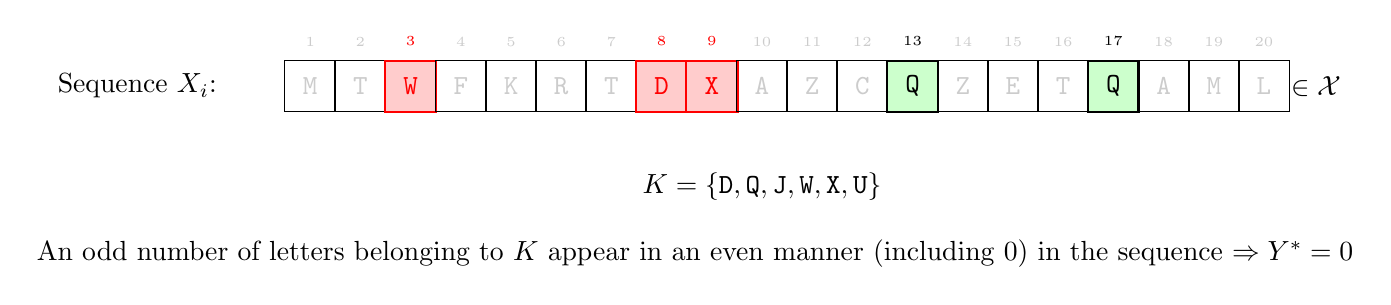
\begin{tikzpicture}[scale=0.85, baseline=(current bounding box.center)]
\foreach \i/\letter in {1/\texttt{M},2/\texttt{T},3/\texttt{W},4/\texttt{F},5/\texttt{K},6/\texttt{R},7/\texttt{T},8/\texttt{D},9/\texttt{X},10/\texttt{A},11/\texttt{Z},12/\texttt{C},13/\texttt{Q},14/\texttt{Z},15/\texttt{E},16/\texttt{T},17/\texttt{Q},18/\texttt{A},19/\texttt{M},20/\texttt{L}} {
    \ifnum\i=3
        \node[draw,thick,red,minimum size=0.65cm,fill=red!20] (n\i) at (\i*0.75,0) {\textbf{\letter}};
    \else
        % D at position 8 (odd count -> red)
        \ifnum\i=8
            \node[draw,thick,red,minimum size=0.65cm,fill=red!20] (n\i) at (\i*0.75,0) {\textbf{\letter}};
        \else
            % U at position 9 (odd count -> red)
            \ifnum\i=9
                \node[draw,thick,red,minimum size=0.65cm,fill=red!20] (n\i) at (\i*0.75,0) {\textbf{\letter}};
            \else
                % Q at positions 13 and 17 (even count -> green)
                \pgfmathparse{\i==13 || \i==17 ? 1 : 0}
                \ifnum\pgfmathresult=1
                    \node[draw,thick,black,minimum size=0.65cm,fill=green!20] (n\i) at (\i*0.75,0) {\textbf{\letter}};
                \else
                    % Non-key letters in gray
                    \node[draw,minimum size=0.65cm,text=gray!40] (n\i) at (\i*0.75,0) {\letter};
                \fi
            \fi
        \fi
    \fi
}
\node[anchor=east] at (-0.5,0) {Sequence $X_i$:};
\node[right=12cm of n1] {$\in \mathcal{X}$};

% Position numbers above letters
\foreach \i in {1,...,20} {
    \pgfmathparse{\i==3 || \i==8 || \i==9 ? "red" : (\i==13 || \i==17 ? "black" : "gray!40")}
    \edef\nodecolor{\pgfmathresult}
    \node[above=0.05cm of n\i,\nodecolor,font=\tiny] {\i};
}

% Key information
\node at (7.5,-1.5) {$K = \{\texttt{D}, \texttt{Q}, \texttt{J}, \texttt{W}, \texttt{X}, \texttt{U}\}$};


% Result
\node[align=center] at (6.5,-2.5) {An odd number of letters belonging to $K$ appear in an even manner (including 0) in the sequence
$\Rightarrow Y^{*}=0$};

\end{tikzpicture}%
}
\caption{Sequence classification example for the \textbf{GPC} mechanism. The parity-relevant subset is $K = \{\texttt{D}, \texttt{Q}, \texttt{J}, \texttt{W}, \texttt{X}, \texttt{U}\}$.
The parity criterion requires \emph{an even number of unique} key letter to appear an \textbf{even} number of times (including 0, which is even).
In green: key letters with even count. In red: key letters with odd count. Note: that also \texttt{J} and \texttt{U} have even count, including zero, in the sequence satisfying Definition~\ref{def:parity}. So we have in total 3 letters in $K$ with an even count, and since 3 is not even the sequence is labeled as $Y^{*}=0$.}
\label{fig:parity_example}
\end{figure*}

\section{Contiguous \(k\)-gram shortcut analysis}
\label{appendix:k_gram_analysis}

This appendix quantifies how much outcome signal is recoverable from contiguous
local patterns alone. A \(k\)-gram is a contiguous subsequence
\((X_t,\ldots,X_{t+k-1})\). For each \(k\)-gram \(g\) observed in the training set,
we estimate \(\hat p(g)=\#(g,Y=1)/\#(g)\). For a test sequence \(X\), we score
\[
s_k(X)=\frac{1}{n-k+1}\sum_{t=1}^{n-k+1}
\hat p(X_t,\ldots,X_{t+k-1}).
\]
Unseen \(k\)-grams are assigned the training-set positive rate. We report AUC,
rather than threshold-dependent metrics, because AUC is the primary metric for
latent-rule recovery.

Table~\ref{tab:ngram_appendix} shows that contiguous \(k\)-grams capture
nontrivial local signal in the compliance tasks but do not reach the neural or
lag-aware pair-count ceiling. In OC-Deterministic, the best contiguous
\(k\)-gram score is around \(0.82\) AUC; in OC-Noisy it is around \(0.59\),
near the smaller decoder-only models. In contrast, all contiguous \(k\)-gram
scores remain at chance on hidden-subset parity. Coverage collapses for
\(k\ge5\), so longer contiguous patterns are too sparse to provide reliable
generalization in this regime.

\begin{table}[tb]
\centering
\small
\caption{
Contiguous \(k\)-gram baseline. Coverage is the fraction of test \(k\)-grams
observed in the training set. OC and GPC mechanisms share the same i.i.d. sequence
proposal, so coverage is common across these tasks.
}
\label{tab:ngram_appendix}
\fitwidth{%
\begin{tabular}{lcccc}
\toprule
\(k\) & Coverage & OC-Deterministic AUC & OC-Noisy AUC & GPC-Deterministic AUC \\
\midrule
1 & 100.0\% & .813 & .585 & .502 \\
2 & 100.0\% & .819 & .586 & .498 \\
3 & 100.0\% & .818 & .576 & .497 \\
4 & 100.0\% & .781 & .534 & .499 \\
5 & 41.7\%  & .617 & .508 & .497 \\
6 & 1.9\%   & .524 & .499 & .501 \\
7 & 0.1\%   & .501 & .501 & .500 \\
\bottomrule
\end{tabular}}
\end{table}

Table~\ref{tab:signal_decomposition} separates content-only, contiguous-local,
and lag-aware signal. The key finding is that contiguous \(k\)-grams explain part
of the compliance performance but not the ceiling: the ceiling is reached only
after exposing the \(\lambda\)-aware pair-count feature.

\begin{table}[tb]
\centering
\small
\caption{
Signal decomposition by feature family, measured by test AUC.
}
\label{tab:signal_decomposition}
\fitwidth{%
\begin{tabular}{lccc}
\toprule
Method & OC-Deterministic & OC-Noisy & GPC-Deterministic \\
\midrule
Chance & .500 & .500 & .500 \\
BoE-key counts & .774 & .574 & .503 \\
BoE-XGB counts & .816 & .584 & .503 \\
Best contiguous \(k\)-gram & .819 & .586 & .502 \\
\(\lambda\)-aware pair LR & .997 & .671 & --- \\
Best neural model & .999 & .671 & .503 \\
Oracle AUC & 1.000 & .670 & 1.000 \\
\bottomrule
\end{tabular}}
\end{table}

\FloatBarrier

\section{Proofs}
\label{appendix:proof_theorems}

\begin{theorem}[Optimal Performance under Label Noise]
\label{thm:optimal_performance}
Under symmetric label noise with parameter $\pi \in [0, 0.5)$ and compliance rate $\rho$ (i.e., $\mathbb{P}(Y^{*}=1)=\rho, \text{ and } \mathbb{P}(Y=1|Y^{*}=1)=1-\pi)$, a classifier with perfect access to compliance status (oracle) achieves:
\[
\mathrm{AUC}^* = \frac{1}{2} + \frac{1}{2}(A - C) \overset{\rho=0.5}{=} 1 - \pi
\]
where
\[
A = \frac{(1-\pi)\rho}{\rho(1-\pi) + (1-\rho)\pi}, \quad C = \frac{\pi\rho}{\rho\pi + (1-\rho)(1-\pi)}.
\]
Similarly, $F_1^* = 2(1-\pi)\rho / (\pi + 2\rho(1-\pi)) \overset{\rho=0.5}{=} 1-\pi$. Per dataset, this gives $\mathrm{AUC}^*=F_1^*=1.000$ for Naive sanity check, OC-Deterministic, and GPC-Deterministic (all with $\pi=0$), and $\mathrm{AUC}^*=0.670$, $F_1^*=0.577$, Precision$^*=0.700$, Recall$^*=0.491$ for OC-Noisy ($\pi=0.3$, $\rho=0.293$).
\end{theorem}

\begin{proof}[Proof of Theorem~\ref{thm:optimal_performance}]
\label{proof:optimal_performance}
Under symmetric label noise,
\[
P(Y=1 \mid Y^{*}=1)=1-\pi, \qquad P(Y=1 \mid Y^{*}=0)=\pi.
\]
Because $\pi < 1/2$, the posterior $P(Y=1 \mid Y^{*})$ is strictly increasing in $Y^{*}$, so any Bayes-optimal ranking is equivalent to scoring by $s=Y^{*}$. We therefore compute the AUC of the binary oracle score $s \in \{0,1\}$.

\begin{equation}
AUC = P(s_+ > s_-) + \frac{1}{2} P(s_+ = s_-)
\end{equation}
where $s_+$ is the score for a random instance with $Y = 1$ and $s_-$ is the score for a random instance with $Y = 0$.

The Joint Distribution is:

\begin{align}
P(Y = 1, Y^* = 1) &= (1-\pi)\rho \\
P(Y = 1, Y^* = 0) &= \pi(1-\rho) \\
P(Y = 0, Y^* = 1) &= \pi\rho \\
P(Y = 0, Y^* = 0) &= (1-\pi)(1-\rho)
\end{align}

Marginal Distributions:

\begin{align}
P(Y = 1) &= \rho(1-\pi) + (1-\rho)\pi \\
P(Y = 0) &= \rho \pi + (1-\rho)(1-\pi)
\end{align}

Note that $P(Y = 1) + P(Y = 0) = 1$.

For the conditional score distributions, define:
\begin{align}
    A &= P(s = 1 \mid Y = 1) = \frac{(1-\pi)\rho}{\rho(1-\pi) + (1-\rho)\pi} \\
    B &= P(s = 0 \mid Y = 1) = \frac{\pi(1-\rho)}{\rho(1-\pi) + (1-\rho)\pi} \\
    C &= P(s = 1 \mid Y = 0) = \frac{\pi\rho}{\rho \pi + (1-\rho)(1-\pi)} \\
    D &= P(s = 0 \mid Y = 0) = \frac{(1-\pi)(1-\rho)}{\rho \pi + (1-\rho)(1-\pi)}
\end{align}


    

Note that $A + B = 1$ and $C + D = 1$.

AUC Calculation:

\begin{align}
AUC &= A \cdot D + \frac{1}{2}(A \cdot C + B \cdot D) \\
&= A(1-C) + \frac{1}{2}A \cdot C + \frac{1}{2}(1-A)(1-C) \\
&= A - AC + \frac{1}{2}AC + \frac{1}{2} - \frac{1}{2}A - \frac{1}{2}C + \frac{1}{2}AC \\
&= \frac{1}{2} + \frac{1}{2}(A - C)
\end{align}

Simplification for balanced classes:

For $\rho = 0.5$:
\begin{align}
A &= \frac{0.5(1-\pi)}{0.5(1-\pi) + 0.5\pi} = \frac{0.5(1-\pi)}{0.5} = 1-\pi \\
C &= \frac{0.5\pi}{0.5\pi + 0.5(1-\pi)} = \frac{0.5\pi}{0.5} = \pi
\end{align}

Therefore:
\begin{equation}
AUC = \frac{1}{2} + \frac{1}{2}[(1-\pi) - \pi] = \frac{1}{2} + \frac{1}{2}(1-2\pi) = 1 - \pi
\end{equation}

Alternatively, we can use the following expression.

Define $X = \rho(1-\pi) + (1-\rho)\pi$ and $Y = \rho \pi + (1-\rho)(1-\pi)$.

The numerator of $(A - C)$ can be computed as:
\begin{align}
(A - C) \cdot XY &= (1-\pi)\rho \cdot Y - \pi\rho \cdot X \\
&= \rho[(1-\pi)Y - \pi X] \\
&= \rho[(1-\pi)(\rho \pi + (1-\rho)(1-\pi)) \\
&\qquad - \pi(\rho(1-\pi) + (1-\rho)\pi)] \\
&= \rho[(1-\pi)^2(1-\rho) - \pi^2(1-\rho)] \\
&= \rho(1-\rho)[(1-\pi)^2 - \pi^2] \\
&= \rho(1-\rho)(1-2\pi)
\end{align}

Note: $(1-\pi)^2 - \pi^2 = 1 - 2\pi + \pi^2 - \pi^2 = 1 - 2\pi$.

Therefore:
\begin{equation}
A - C = \frac{\rho(1-\rho)(1-2\pi)}{XY}
\end{equation}

and
\begin{equation}
AUC = \frac{1}{2} + \frac{\rho(1-\rho)(1-2\pi)}{2XY}
\end{equation}
\qed

For the thresholded oracle classifier $\widehat{Y}=Y^{*}$, we now compute the resulting F1 score with respect to the observed labels.

Since we evaluate performance against the stochastic observed labels $Y$, the confusion matrix elements are:

\begin{align}
\text{TP} &= P(\hat{Y} = 1 \cap Y = 1) = P(Y^* = 1 \cap Y = 1) \nonumber \\
&= P(Y = 1 \mid Y^* = 1) \cdot P(Y^* = 1) = (1-\pi)\rho \\
\text{FP} &= P(\hat{Y} = 1 \cap Y = 0) = P(Y^* = 1 \cap Y = 0) \nonumber \\
&= P(Y = 0 \mid Y^* = 1) \cdot P(Y^* = 1) = \pi\rho \\
\text{FN} &= P(\hat{Y} = 0 \cap Y = 1) = P(Y^* = 0 \cap Y = 1) \nonumber \\
&= P(Y = 1 \mid Y^* = 0) \cdot P(Y^* = 0) = \pi(1-\rho) \\
\text{TN} &= P(\hat{Y} = 0 \cap Y = 0) = P(Y^* = 0 \cap Y = 0) \nonumber \\
&= P(Y = 0 \mid Y^* = 0) \cdot P(Y^* = 0) = (1-\pi)(1-\rho)
\end{align}

For the precision, by definition:
\begin{align}
\text{Precision} &= \frac{\text{TP}}{\text{TP} + \text{FP}} = \frac{(1-\pi)\rho}{(1-\pi)\rho + \pi\rho} \nonumber \\
&= \frac{(1-\pi)\rho}{\rho[(1-\pi) + \pi]} = \frac{(1-\pi)\rho}{\rho} = 1 - \pi
\end{align}

\textbf{Observation:} Precision is independent of the class distribution $\rho$ and depends only on the noise rate $\pi$.

For the recall, by definition:
\begin{align}
\text{Recall} &= \frac{\text{TP}}{\text{TP} + \text{FN}} = \frac{(1-\pi)\rho}{(1-\pi)\rho + \pi(1-\rho)} \nonumber \\
&= \frac{(1-\pi)\rho}{\rho - \pi\rho + \pi - \pi\rho} = \frac{(1-\pi)\rho}{\rho(1-2\pi) + \pi}
\end{align}

\textbf{Verification for $\rho = 0.5$:}
\begin{equation}
\begin{aligned}
\text{Recall}
&= \frac{(1-\pi) \cdot 0.5}{0.5(1-2\pi) + \pi}
 = \frac{0.5(1-\pi)}{0.5 - \pi + \pi} \\
&= \frac{0.5(1-\pi)}{0.5} = 1 - \pi
\end{aligned}
\end{equation}

Thus, for balanced classes, precision $=$ recall $= 1-\pi$.

For F1, we use the harmonic mean of precision and recall:
\begin{equation}
F_1 = \frac{2 \cdot \text{Precision} \cdot \text{Recall}}{\text{Precision} + \text{Recall}}
\end{equation}

Substituting our expressions:
\begin{align}
F_1 &= \frac{2(1-\pi) \cdot \frac{(1-\pi)\rho}{\rho(1-2\pi) + \pi}}{(1-\pi) + \frac{(1-\pi)\rho}{\rho(1-2\pi) + \pi}} \nonumber \\
&= \frac{2(1-\pi)^2\rho}{(1-\pi)[\rho(1-2\pi) + \pi] + (1-\pi)\rho}
\end{align}

Simplifying the denominator:
\begin{align}
&(1-\pi)[\rho(1-2\pi) + \pi] + (1-\pi)\rho \nonumber \\
&= (1-\pi)\rho(1-2\pi) + \pi(1-\pi) + (1-\pi)\rho \nonumber \\
&= (1-\pi)\rho[(1-2\pi) + 1] + \pi(1-\pi) \nonumber \\
&= (1-\pi)\rho(2-2\pi) + \pi(1-\pi) \nonumber \\
&= (1-\pi)[2\rho(1-\pi) + \pi]
\end{align}

Therefore:
\begin{align}
F_1 &= \frac{2(1-\pi)^2\rho}{(1-\pi)[2\rho(1-\pi) + \pi]} = \frac{2(1-\pi)\rho}{2\rho(1-\pi) + \pi} \nonumber \\
&= \frac{2(1-\pi)\rho}{\pi + 2\rho(1-\pi)}
\end{align}

\textbf{Verification for $\rho = 0.5$:}
\begin{equation}
\begin{aligned}
F_1 &= \frac{2(1-\pi) \cdot 0.5}{\pi + 2 \cdot 0.5 \cdot (1-\pi)} \\
&= \frac{1-\pi}{\pi + (1-\pi)} = \frac{1-\pi}{1} = 1 - \pi
\end{aligned}
\end{equation}

\end{proof}

\subsection{Proof of Theorem~\ref{thm:impossibility}}
\label{appendix:proof_impossibility}

\begin{proof}
Let $s_{\min}\in\mathcal{S}$ satisfy $\kappa(s_{\min})=1$.
We first show that the map
\[
a \longmapsto P(Y^*=1\mid X_1=a)
\]
is not constant on $\mathcal{A}$.

\paragraph{Case 1: $\mathcal{S}\subsetneq\mathcal{A}$.}
Choose $a_0\in\mathcal{A}\setminus\mathcal{S}$.
Because the coordinates of $X$ are independent and have full support,
both events $\{X_1=s_{\min}\}$ and $\{X_1=a_0\}$ have positive probability,
and conditioning on $X_1$ does not change the joint law of
$(X_2,\ldots,X_n)$.

Let $Z_2,\ldots,Z_n$ be independent random variables with
$Z_t\sim\mathcal{L}(X_t)$, and define
\[
\widetilde X := (s_{\min},Z_2,\ldots,Z_n),
\qquad
\widetilde X' := (a_0,Z_2,\ldots,Z_n).
\]
Then
\[
\widetilde X \stackrel{d}{=} (X\mid X_1=s_{\min}),
\qquad
\widetilde X' \stackrel{d}{=} (X\mid X_1=a_0).
\]

Let
\[
C := \{\widetilde X \text{ is compliant}\},
\qquad
C' := \{\widetilde X' \text{ is compliant}\}.
\]
Since $\widetilde X'_1=a_0\notin\mathcal S$, any ordered maximal
$\lambda$-run in $\widetilde X'$ must avoid position $1$. If such a run does
not start at $1+\lambda$, the same maximal run is present in $\widetilde X$.
If it starts at $1+\lambda$, then in $\widetilde X$ it is extended to the left
by $s_{\min}$, and the extended maximal run remains ordered because
$\kappa(s_{\min})=1$ is the minimum rank. Hence every compliant witness in
$\widetilde X'$ induces a compliant witness in $\widetilde X$, so
\[
C'\subseteq C.
\]

Now define the event
\[
E
:=
\{Z_{1+\lambda}\in\mathcal{S}\}
\cap
\bigcap_{t\in\{2,\ldots,n\}\setminus\{1+\lambda\}}
\{Z_t\notin\mathcal{S}\}.
\]
Because $n\ge \lambda+1$, because $\mathcal{S}\subsetneq\mathcal{A}$,
and because every symbol has positive probability at every position,
we have $P(E)>0$.

On $E$, the sequence $\widetilde X$ contains the maximal $\lambda$-run
$(1,1+\lambda)$: both symbols belong to $\mathcal S$, the gap is $\lambda$,
the run cannot be extended to the left, and it cannot be extended to the right
because all other positions are non-key. Moreover,
\[
\kappa(\widetilde X_1)=\kappa(s_{\min})=1
\leq
\kappa(\widetilde X_{1+\lambda}).
\]
Hence this maximal run is ordered, and $\widetilde X$ is compliant.

On the same event $E$, the sequence $\widetilde X'$ is not compliant.
Indeed, among positions $2,\ldots,n$, the only key position is $1+\lambda$,
so no compliant chain of length at least $2$ can exist. Therefore
\[
E \subseteq C\setminus C'.
\]

Since \(C' \subseteq C\), we have
\[
P(C)-P(C') = P(C\setminus C').
\]
Moreover, \(E \subseteq C\setminus C'\) and \(P(E)>0\). Therefore
\[
P(C)-P(C') \ge P(E) > 0,
\]
which implies
\[
P(C) > P(C').
\]
Hence
\[
\begin{aligned}
P(Y^*=1 \mid X_1=s_{\min})
&=
P(C)
>
P(C')\\
&=
P(Y^*=1 \mid X_1=a_0).
\end{aligned}
\]

\paragraph{Case 2: $\mathcal{S}=\mathcal{A}$.}
When $\mathcal{S}=\mathcal{A}$, the maximal $\lambda$-runs are deterministic:
they are the residue classes of positions modulo $\lambda$, truncated to
$\{1,\ldots,n\}$. Let
\[
L := 1+\left\lfloor \frac{n-1}{\lambda}\right\rfloor .
\]
Since $n\geq \lambda+1$, we have $L\geq 2$. Let
\[
R_1 := (1,1+\lambda,\ldots,1+(L-1)\lambda)
\]
be the maximal $\lambda$-run containing position $1$.

Let $O_1$ be the event that $R_1$ is ordered, and let $B$ be the event that
some maximal $\lambda$-run different from $R_1$ is ordered. Then
\[
\{Y^*=1\}=B\cup O_1.
\]
Moreover, $B$ depends only on coordinates outside $R_1$, whereas $O_1$
depends only on coordinates in $R_1$. By independence of the coordinates,
for every $a\in\mathcal{A}$,
\[
\begin{aligned}
&P(Y^*=1\mid X_1=a)\\
&\qquad=
P(B)+(1-P(B))\,P(O_1\mid X_1=a).
\end{aligned}
\]
Since $B\subseteq\{Y^*=1\}$, if $P(B)=1$ then $P(Y^*=1)=1$, contradicting
$\rho\in(0,1)$. Hence
\[
P(B)<1.
\]

Let $s_{\max}\in\mathcal{A}$ satisfy
\[
\kappa(s_{\max})=|\mathcal{A}|.
\]
The assumption $\rho\in(0,1)$ implies $|\mathcal{A}|\geq 2$, so
$s_{\min}\neq s_{\max}$. Define
\[
p_a := P(O_1\mid X_1=a).
\]
We now show that $p_{s_{\min}}>p_{s_{\max}}$.

Conditioning on $X_1=s_{\min}$, the first element of $R_1$ has minimal
rank. Thus
\[
\begin{aligned}
p_{s_{\min}}
=
P\bigl(
&\kappa(X_{1+\lambda})
\leq
\kappa(X_{1+2\lambda})\\
&\leq
\cdots
\leq
\kappa(X_{1+(L-1)\lambda})
\bigr),
\end{aligned}
\]
with the convention that the event is the whole space when $L=2$.
Conditioning on $X_1=s_{\max}$, the first element of $R_1$ has maximal rank,
so the run can be ordered only if every later element of the run is also
$s_{\max}$:
\[
p_{s_{\max}}
=
P\!\left(
X_{1+\lambda}=X_{1+2\lambda}=\cdots=X_{1+(L-1)\lambda}=s_{\max}
\right).
\]
The latter event is contained in the former. The containment is strict with
positive probability, because by full support and independence the event
\[
X_{1+\lambda}=X_{1+2\lambda}=\cdots=X_{1+(L-1)\lambda}=s_{\min}
\]
has positive probability, belongs to the former event, and does not belong to
the latter. Therefore
\[
p_{s_{\min}}>p_{s_{\max}}.
\]
Consequently,
\begin{align*}
&P(Y^*=1\mid X_1=s_{\min})
-
P(Y^*=1\mid X_1=s_{\max})
\\
&\qquad =
(1-P(B))\,(p_{s_{\min}}-p_{s_{\max}})
>0.
\end{align*}
Thus
\[
P(Y^*=1\mid X_1=s_{\min})
\neq
P(Y^*=1\mid X_1=s_{\max}).
\]

In both cases, there exist $a,b\in\mathcal{A}$ such that
\[
P(Y^*=1\mid X_1=a)\neq P(Y^*=1\mid X_1=b).
\]
Therefore $Y^*$ is not independent of $X_1$. Since mutual information
between discrete variables is zero if and only if the variables are
independent, it follows that
\[
I(Y^*;X_1)>0.
\]

Finally, by the symmetric noise model \eqref{eq:label_noise},
\begin{align*}
&P(Y=1\mid X_1=a)\\
&=
P(Y=1\mid Y^*=1)\,P(Y^*=1\mid X_1=a)
\\
&\quad+
P(Y=1\mid Y^*=0)\,P(Y^*=0\mid X_1=a)
\\
&=
(1-\pi)\,P(Y^*=1\mid X_1=a)\\
&\quad+
\pi\,\bigl(1-P(Y^*=1\mid X_1=a)\bigr)
\\
&=
\pi + (1-2\pi)\,P(Y^*=1\mid X_1=a).
\end{align*}
Because $\pi<1/2$, the map
\[
u \longmapsto \pi + (1-2\pi)u
\]
is strictly increasing. Hence the map
\[
a \longmapsto P(Y=1\mid X_1=a)
\]
is also non-constant on $\mathcal{A}$. Thus $Y$ is not independent of $X_1$,
and again
\[
I(Y;X_1)>0.
\]
\end{proof}

\subsection{A Quantitative Uniform Lower Bound}
\label{sec:uniform_witness_bound}

Theorem~\ref{thm:impossibility} is qualitative and holds under independent full-support sampling. Under the uniform proposal law used in our synthetic benchmark, the witness event in its proof yields an explicit lower bound on the amount of local leakage.

\begin{corollary}[Uniform witness lower bound]
\label{cor:uniform_witness_bound}
Assume the setting of Theorem~\ref{thm:impossibility} with
$\mathcal{S}\subsetneq\mathcal{A}$ and
$X_t \overset{\mathrm{iid}}{\sim} \mathrm{Uniform}(\mathcal{A})$.
Let $s_{\min}\in\mathcal{S}$ satisfy $\kappa(s_{\min})=1$ and
$a_0\in\mathcal{A}\setminus\mathcal{S}$. Define
$\delta(a,b) := P(Y^*\!=\!1\mid X_1\!=\!a)
              - P(Y^*\!=\!1\mid X_1\!=\!b)$.
Then
\begin{equation}
\label{eq:witness_clean}
\delta(s_{\min},a_0)
\;\ge\;
\frac{m}{\ell}
\!\left(\frac{\ell-m}{\ell}\right)^{\!n-2}.
\end{equation}
If $Y$ is generated from $Y^*$ via \eqref{eq:label_noise}, then
\begin{equation}
\label{eq:witness_noisy}
\delta_Y(s_{\min},a_0)
\;\ge\;
(1-2\pi)\,\frac{m}{\ell}
\!\left(\frac{\ell-m}{\ell}\right)^{\!n-2},
\end{equation}
where
$\delta_Y(a,b) := P(Y\!=\!1\mid X_1\!=\!a)
                 - P(Y\!=\!1\mid X_1\!=\!b)$.
\end{corollary}

See \ref{appendix:proof_uniform_witness_bound} for full proof and remarks.




\subsection{Proof of Corollary~\ref{cor:uniform_witness_bound} with remarks}
\label{appendix:proof_uniform_witness_bound}
\begin{proof}
As in the proof of Theorem~\ref{thm:impossibility}, let
$Z_2,\ldots,Z_n$ be independent random variables with
$Z_t\sim \mathrm{Uniform}(\mathcal{A})$, and define
\[
\widetilde X=(s_{\min},Z_2,\ldots,Z_n),
\qquad
\widetilde X'=(a_0,Z_2,\ldots,Z_n).
\]
Then
\[
\widetilde X \stackrel{d}{=} (X\mid X_1=s_{\min}),
\qquad
\widetilde X' \stackrel{d}{=} (X\mid X_1=a_0).
\]

Let
\[
C:=\{\widetilde X \text{ is compliant}\},
\qquad
C':=\{\widetilde X' \text{ is compliant}\}.
\]
As in Theorem~\ref{thm:impossibility}, one has $C'\subseteq C$.

Now define the witness event
\[
E
:=
\{Z_{1+\lambda}\in\mathcal{S}\}
\cap
\bigcap_{t\in\{2,\ldots,n\}\setminus\{1+\lambda\}}
\{Z_t\notin\mathcal{S}\}.
\]
On $E$, the sequence $\widetilde X$ is compliant via the chain
$(1,1+\lambda)$, while $\widetilde X'$ is not compliant. Hence
\[
E \subseteq C\setminus C'.
\]
Therefore
\[
P(C)-P(C') = P(C\setminus C') \ge P(E).
\]

By independence and uniformity,
\[
\begin{aligned}
&P(Z_{1+\lambda}\in\mathcal{S})=\frac{m}{\ell},
\qquad
P(Z_t\notin\mathcal{S})=\frac{\ell-m}{\ell}\\
&\text{for each } t\in\{2,\ldots,n\}\setminus\{1+\lambda\}.
\end{aligned}
\]
There are exactly $n-2$ such latter positions, so
\[
P(E)
=
\frac{m}{\ell}\left(\frac{\ell-m}{\ell}\right)^{n-2}.
\]
Since
\[
\begin{aligned}
P(C)&=P(Y^*=1\mid X_1=s_{\min}),\\
P(C')&=P(Y^*=1\mid X_1=a_0),
\end{aligned}
\]
the first claim follows.

For the observed label, by \eqref{eq:label_noise},
\[
P(Y=1\mid X_1=a)
=
\pi + (1-2\pi)\,P(Y^*=1\mid X_1=a).
\]
Subtracting the expressions for $a=s_{\min}$ and $a=a_0$ yields
\[
P(Y=1\mid X_1=s_{\min})
-
P(Y=1\mid X_1=a_0)
=
\]
\[
\begin{aligned}
= (1-2\pi)\Bigl(
&P(Y^*=1\mid X_1=s_{\min})\\
&-
P(Y^*=1\mid X_1=a_0)
\Bigr),
\end{aligned}
\]
and the result follows from the first part.
\end{proof}

\begin{remark}[Scope of the explicit bound]
\label{rem:scope_uniform_bound}
The closed-form expression in Corollary~\ref{cor:uniform_witness_bound} is
specific to the uniform proposal law. Under the more general assumptions of
Theorem~\ref{thm:impossibility}, if we write
\[
\alpha_t := P(X_t\in\mathcal{S}),
\]
then the same witness-event argument gives
\[
\begin{aligned}
&P(Y^*=1\mid X_1=s_{\min})
-
P(Y^*=1\mid X_1=a_0)\\
&\qquad\;\ge\;
\alpha_{1+\lambda}
\prod_{t\in\{2,\ldots,n\}\setminus\{1+\lambda\}}(1-\alpha_t)
\end{aligned}
\]
whenever $\mathcal{S}\subsetneq\mathcal{A}$.
In the i.i.d.\ but non-uniform case with common law $q$, this becomes
\[
q(\mathcal{S})\bigl(1-q(\mathcal{S})\bigr)^{n-2}.
\]
No nontrivial positive lower bound depending only on $(m,\ell,n)$ can hold under
mere full support, since $q(\mathcal{S})$ can be arbitrarily small while
remaining positive.
\end{remark}

\begin{remark}[Effect of label balancing]
\label{rem:label_balancing}
Suppose the final experimental sample is obtained from a proposal law $P$ by
retaining examples with probability depending only on the observed label $Y$.
Equivalently,
\[
Q(x,y)=\frac{r_y P(x,y)}{Z},
\qquad r_0,r_1>0.
\]
Then
\[
Q(X\mid Y=y)=P(X\mid Y=y),
\]
so class-conditional sequence structure, and hence AUC, are unchanged by this
reweighting. However, posterior quantities are transformed. Writing
$\beta:=r_1/r_0$ and
\[
h_\beta(u):=\frac{\beta u}{1+(\beta-1)u},
\]
one has
\[
Q(Y=1\mid X_1=a)
=
h_\beta\!\bigl(P(Y=1\mid X_1=a)\bigr).
\]
Since $h_\beta$ is strictly increasing, label balancing preserves the presence of
local information, but because $h_\beta$ is nonlinear it can either enlarge or
shrink posterior gaps. Consequently,
Corollary~\ref{cor:uniform_witness_bound} should be interpreted as a statement
about the proposal law, not automatically about the retained balanced sample.

More generally, if
\[
\Delta_P := P(Y=1\mid X_1=s_{\min}) - P(Y=1\mid X_1=a_0),
\]
\[
\Delta_Q := Q(Y=1\mid X_1=s_{\min}) - Q(Y=1\mid X_1=a_0),
\]
Then by the mean value theorem:
\[
\Delta_Q \ge \min\{\beta,\beta^{-1}\}\,\Delta_P.
\]
The same remark applies with $Y^*$ in place of $Y$ if balancing is performed
using the latent label rather than the observed one.
\end{remark}



\subsection{Proof of Theorem~\ref{thm:parity_local_purity}}
\label{appendix:proof_parity_local_purity}

\begin{proof}
For each \(t\in\{1,\ldots,n\}\), define
\[
B_t := \mathbf{1}\{X_t\in K\}.
\]
Since \(X_t \overset{\mathrm{iid}}{\sim} \mathrm{Uniform}(\mathcal A)\) and
\[
p = \frac{|K|}{|\mathcal A|},
\]
we have
\[
B_t \overset{\mathrm{iid}}{\sim} \mathrm{Bernoulli}(p).
\]
Let
\[
T := \Bigl(\sum_{t=1}^n B_t\Bigr)\bmod 2.
\]

We first show that \(Y^*\) is a fixed bit-flip of \(T\). Using addition modulo \(2\),
\[
\mathbf{1}\{N_k \text{ is even}\} = 1 \oplus (N_k \bmod 2),
\]
where \(\oplus\) denotes XOR. Hence

\begin{align*}
Y^*
&=
1 \oplus\bigoplus_{k\in K} \mathbf{1}\{N_k \text{ is even}\} \\
&=
1 \oplus\bigoplus_{k\in K} \bigl(1 \oplus (N_k \bmod 2)\bigr) \\
&=
1 \oplus\bigl(|K|\bmod 2\bigr)\oplus \bigoplus_{k\in K}(N_k \bmod 2).
\end{align*}
But
\[
\begin{aligned}
\bigoplus_{k\in K}(N_k \bmod 2)
&=
\Bigl(\sum_{k\in K} N_k\Bigr)\bmod 2\\
&=
\Bigl(\sum_{t=1}^n \mathbf{1}\{X_t\in K\}\Bigr)\bmod 2
=
T.
\end{aligned}
\]
Therefore
\[
Y^* = 1 \oplus\bigl(|K|\bmod 2\bigr)\oplus T.
\]
The map \(T\mapsto Y^*\) is thus a bijection on \(\{0,1\}\), so for every index set \(J\),
\[
I(Y^*;X_J)=I(T;X_J).
\]
It is therefore enough to study \(I(T;X_J)\).

Fix an index set
\[
J\subseteq \{1,\ldots,n\},
\qquad 1\le |J|<n.
\]
Write
\[
r := |J|,
\qquad
s := n-r = |J^c| \ge 1.
\]
Define
\[
U_J := \Bigl(\sum_{j\in J} B_j\Bigr)\bmod 2,
\qquad
V_J := \Bigl(\sum_{j\in J^c} B_j\Bigr)\bmod 2.
\]
Then
\[
T = U_J \oplus V_J.
\]

Since \(\{B_j : j\in J\}\) and \(\{B_j : j\in J^c\}\) are independent,
\(V_J\) is independent of \(X_J\). Moreover, \(U_J\) is a deterministic function of
\(X_J\).

Let
\[
q_s := P(V_J=1).
\]
Because \(V_J\) is the parity of \(s\) i.i.d.\ Bernoulli\((p)\) random variables,
\[
q_s = \frac{1-(1-2p)^s}{2}.
\]
Therefore, for every realization \(x_J\) of \(X_J\),
\[
P(T=1\mid X_J=x_J)
=
\begin{cases}
q_s, & U_J(x_J)=0,\\
1-q_s, & U_J(x_J)=1.
\end{cases}
\]

\paragraph{Balanced case: \(p=1/2\).}
If \(p=1/2\), then
\[
q_s = \frac{1-(1-2p)^s}{2} = \frac{1}{2}.
\]
Hence, for every realization \(x_J\),
\[
\begin{aligned}
P(T=1\mid X_J=x_J)&=\tfrac12,\\
P(T=0\mid X_J=x_J)&=\tfrac12.
\end{aligned}
\]
Thus the conditional law of \(T\) does not depend on \(x_J\), so \(T\) is independent
of \(X_J\). Therefore
\[
I(T;X_J)=0,
\]
and hence
\[
I(Y^*;X_J)=0.
\]

\paragraph{Unbalanced case: \(p\neq 1/2\), finite \(n\).}
Since \(K\) is nonempty and proper, \(p\in(0,1)\). If \(p\neq 1/2\), then
\[
|1-2p|<1
\qquad\text{and}\qquad
(1-2p)^s \neq 0
\]
for every finite \(s\ge 1\). Hence
\[
q_s \neq \frac12.
\]

Choose any \(j_0\in J\), any \(a_{\mathrm{in}}\in K\), and any
\(a_{\mathrm{out}}\in \mathcal A\setminus K\). Define two realizations
\(x_J,x'_J\in \mathcal A^J\) by
\[
x_j = a_{\mathrm{out}} \quad \text{for all } j\in J,
\]
and
\[
x'_{j_0}=a_{\mathrm{in}},
\qquad
x'_j=a_{\mathrm{out}} \quad \text{for all } j\in J\setminus\{j_0\}.
\]
Then
\[
U_J(x_J)=0,
\qquad
U_J(x'_J)=1.
\]
Therefore
\[
\begin{aligned}
P(T=1\mid X_J=x_J)&=q_s,\\
P(T=1\mid X_J=x'_J)&=1-q_s.
\end{aligned}
\]
Since \(q_s\neq 1/2\), these two conditional probabilities are different. Thus the
conditional law of \(T\) depends on \(X_J\), so \(T\) and \(X_J\) are not independent.
Hence
\[
I(T;X_J)>0,
\]
and therefore
\[
I(Y^*;X_J)>0.
\]

\paragraph{Asymptotic decay when \(p\neq 1/2\).}
Now let \(J\subset\mathbb N\) be any fixed finite index set, and for all sufficiently large
\(n\) identify it with a subset of \(\{1,\ldots,n\}\). Then \(r=|J|\) is fixed and
\[
s=n-r \to \infty.
\]
Since \(|1-2p|<1\),
\[
q_s = \frac{1-(1-2p)^s}{2} \to \frac12.
\]
Hence, uniformly over all realizations \(x_J\),
\[
P(T=1\mid X_J=x_J)\to \frac12.
\]
Because \(X_J\) takes values in the finite set \(\mathcal A^r\), this implies that the joint
law of \((T,X_J)\) converges to the product law of \(T\) and \(X_J\). Therefore
\[
I(T;X_J)\to 0.
\]
Since \(Y^*\) is a bijective function of \(T\),
\[
I(Y^*;X_J)=I(T;X_J)\to 0.
\]

\paragraph{Observed stochastic label \(Y\).}
Assume now that \(Y\) is generated from \(Y^*\) according to \eqref{eq:label_noise}
with \(\pi<1/2\).

If \(p=1/2\), then \(Y^*\) is independent of \(X_J\). Since \(Y\) depends on \(X_J\)
only through \(Y^*\), it follows that \(Y\) is also independent of \(X_J\). Hence
\[
I(Y;X_J)=0.
\]

If \(p\neq 1/2\), then
\begin{align*}
P(Y=1\mid X_J)
&=
P(Y=1\mid Y^*=1)\,P(Y^*=1\mid X_J) \\
&\quad +
P(Y=1\mid Y^*=0)\,P(Y^*=0\mid X_J) \\
&=
(1-\pi)P(Y^*=1\mid X_J)\\
&\quad+
\pi\bigl(1-P(Y^*=1\mid X_J)\bigr) \\
&=
\pi + (1-2\pi)P(Y^*=1\mid X_J).
\end{align*}
Because \(\pi<1/2\), the map
\[
u \mapsto \pi + (1-2\pi)u
\]
is strictly increasing. Thus whenever \(P(Y^*=1\mid X_J)\) is non-constant as a
function of \(X_J\), so is \(P(Y=1\mid X_J)\). Therefore, for every finite \(n\),
\[
I(Y;X_J)>0.
\]

Finally, since \(Y\) is obtained from \(Y^*\) through a channel independent of \(X_J\),
the data processing inequality gives
\[
I(Y;X_J)\le I(Y^*;X_J).
\]
Hence, for every fixed finite \(J\subset\mathbb N\),
\[
I(Y;X_J)\to 0
\qquad\text{as } n\to\infty.
\]

This proves all claims. In particular, when \(p=1/2\), we have
\[
\begin{aligned}
&I(Y^*;X_J)=0\\
&\text{for every } J\subseteq \{1,\ldots,n\}\text{ with } |J|<n.
\end{aligned}
\]
Therefore the task is \(k\)-locally pure for every \(k<n\).
\end{proof}

% ==================================================
% HYPERPARAMETER CONFIGURATION
% ==================================================

\section{Models and Hyperparameter Configurations}
\label{appendix:training}

This appendix provides complete hyperparameter configurations for all models evaluated in our experiments.

\subsection{Training Procedure}
\label{subsec:training_appendix}

\paragraph{Optimization.}
All neural models are trained using the AdamW optimizer~\citep{AdamW} with weight decay. For pretrained LLMs and BERT, we use a linear learning rate schedule with 6\% warmup steps. We employ cross-entropy loss for binary classification. Training uses early stopping based on validation loss with patience of 3 epochs for pretrained models and 5 epochs for models trained with randomly initialized parameters.

\paragraph{Pretrained models.}
LLMs (Llama, Qwen) and BERT are fine-tuned with learning rate $2 \times 10^{-5}$, batch size 16, and maximum sequence length 200 tokens. To enable efficient fine-tuning, we apply LoRA~\citep{LoRA} with rank $r=8$, $\alpha=16$, and dropout 0.1, targeting the attention projection matrices (\texttt{q\_proj}, \texttt{k\_proj}, \texttt{v\_proj}, \texttt{o\_proj} for LLMs; \texttt{query}, \texttt{key}, \texttt{value} for BERT). Large models employ gradient checkpointing and mixed-precision training (bfloat16) to fit within GPU memory constraints. We train for a maximum of 20 epochs with patience of 3 epochs. Table~\ref{tab:llm_config} summarizes the fine-tuning configuration for pretrained LLMs. Table~\ref{tab:tiny_llm_config} shows the architectural configurations for small-scale Llama models trained with randomly initialized parameters. Table~\ref{tab:bert_config} summarizes the fine-tuning configuration for BERT-based models.

\paragraph{Randomly initialized Models.}
LSTM, BiLSTM, Transformer, and hybrid architectures are trained with batch size 64 for up to 30 epochs. Learning rates are tuned per architecture: $10^{-3}$ for recurrent models (LSTM, BiLSTM), $5 \times 10^{-4}$ for Transformer-based models, and $10^{-4}$ for the RNNTransformer. Dropout rates range from 0.2 to 0.3 depending on model capacity. Early stopping monitors validation F1 score with patience of 5 epochs. Table~\ref{tab:dl_training} summarizes the training configuration shared across all models trained from scratch. Table~\ref{tab:dl_default_config} and Table~\ref{tab:dl_optimal_config} present the default and optimized architecture configurations, respectively.

Additional architecture details:
\begin{itemize}
    \item \textbf{Transformer}: 4 attention heads; GELU activation; learnable positional encodings; mean pooling with padding mask.
    \item \textbf{LSTM}: Final hidden state used for classification.
    \item \textbf{RNNTransformer}: BiLSTM output projected to embedding dimension, then processed by Transformer encoder.
\end{itemize}


\paragraph{XGBoost baselines.}
XGBoost models use learning rate 0.05, maximum depth 6, subsample ratio 0.8, and column sampling ratio 0.8 per tree. We apply L1 regularization ($\alpha=0.5$) and L2 regularization ($\lambda=1.5$) with minimum child weight 2 and minimum split gain $\gamma=0.1$. Class imbalance is addressed via \texttt{scale\_pos\_weight}. Training runs for up to 200 boosting rounds with early stopping (patience 10) based on validation log-loss. Table~\ref{tab:xgboost_config} presents the XGBoost configuration. For XGBoost-LLM, embeddings are extracted from Llama-3.2-1B using the prompt format described in Section~\ref{subsec:encoding}, with mean pooling over the last hidden layer (dimension 2048).

\paragraph{Threshold optimization.}
For all models, we optimize the classification threshold on the validation set by searching over $\{0.10, 0.11, \ldots, 0.89\}$ to maximize F1 score, rather than using the default 0.5 threshold.

\begin{table}[tb]
\centering
\caption{Models tested and relative dimension. For XGBoost, we report hyperparameter configuration in Table~\ref{tab:xgboost_config}. As tree ensemble complexity is not directly comparable to neural network parameter counts, we omit this metric; the trained model typically comprised 80--120 trees with maximum depth 6.}
\label{tab:models}
\fitwidth{%
\begin{tabular}{llr}
\toprule
Category & Model & Parameters \\
\midrule
\multirow{7}{*}{Pretrained}
  & BERT-base & 110M \\
  & RoBERTa & 355M\\
  & Llama-3.2-1B & 1.0B \\
  & Qwen3-4B-Think & 4.0B\\
  & Llama-3.1-8B & 8.0B \\
  & Qwen2.5-14B & 14B \\
  & Llama-3.1-70B & 70B \\
\midrule
\multirow{5}{*}{Randomly initialized}
  & Llama-1M & 1M  \\
  & LSTM & 198K--340K \\
  & BiLSTM & 256K--395K \\
  & Transformer & 103K--104K \\
  & RNNTransformer$^{*}$ & 319K--455K \\
\midrule
Tree-based & XGBoost & -- \\
\bottomrule
\multicolumn{3}{@{}l@{}}{\footnotesize $^{*}$We call RNNTransformer a BiLSTM-Transformer.}
\end{tabular}}
\end{table}


\subsection{Sequence Encoding}
\label{subsec:encoding}
We use three encoding strategies depending on the model family. \textbf{Prompt-based (LLMs and BERT).} For pretrained language models, we convert each sequence into a natural language prompt of the form \texttt{Sequential events: $x_1$ $x_2$ $\cdots$ $x_n$}. 

For causal LLMs (Llama, Qwen), we additionally append the literal string \texttt{Outcome (0 or 1)}: so that the prompt always terminates at a fixed sentinel position; the true label is never appended to the prompt. Fine-tuning combines (i) the standard auto-regressive language-modeling loss on the prompt itself (no label leakage, equivalent to continued pretraining on the letter-sequence template) with (ii) a binary classification loss from a 2-layer MLP head ($d_{\text{model}} \to d_{\text{model}}/2 \to 2$, with Tanh and dropout 0.1) that reads from the last non-padding hidden state. The two losses are summed with equal weight; LoRA adapters cover only the backbone (q/k/v/o\_proj, $r{=}8$), while the classification head is trained full-rank from scratch. At inference and for early-stopping, predictions come from the head's softmax, not from next-token logits. The prompt is then tokenized using each model's native tokenizer. This same prompt format is used to extract embeddings from Llama-3.2-1B for the XGBoost-LLM baseline, where we apply mean pooling over the last hidden layer.

\textbf{Learned and ordinal embeddings.} For all non-pretrained models, we map each letter to an integer index ($\texttt{A} \mapsto 1, \texttt{B} \mapsto 2, \ldots, \texttt{Z} \mapsto 26$). For XGBoost-basic, this ordinal encoding is used directly as features, relying on the tree ensemble to learn sequential dependencies. For neural architectures (LSTM, Transformer, and hybrids), a learned embedding layer maps each index to a dense vector $\mathbf{e}_i \in \mathbb{R}^{d_e}$ with $d_e \in \{32, 64, 128\}$. Transformer-based models additionally incorporate learnable positional encodings $\mathbf{h}_i = \mathbf{e}_i + \mathbf{p}_i$, where $\mathbf{P} \in \mathbb{R}^{L_{\max} \times d_e}$ is initialized from a standard normal distribution. Sequences are zero-padded within each mini-batch.

\begin{table}[tb]
\centering
\caption{Fine-tuning configuration for pretrained LLMs (Llama, Qwen families).}
\label{tab:llm_config}
\fitwidth{%
\begin{tabular}{ll}
\toprule
Hyperparameter & Value \\
\midrule
\multicolumn{2}{l}{\textit{Training}} \\
Learning rate & $2 \times 10^{-5}$ \\
Optimizer & AdamW \\
Batch size & 16 \\
Max epochs & 20 \\
Early stopping patience & 3 \\
Early stopping criterion & Validation loss \\
Warmup ratio & 6\% of total steps \\
Scheduler & Linear decay \\
\midrule
\multicolumn{2}{l}{\textit{LoRA Configuration (backbone only)}} \\
Rank ($r$) & 8 \\
Alpha ($\alpha$) & 16 \\
Dropout & 0.1 \\
Target modules & \texttt{q\_proj}, \texttt{k\_proj}, \texttt{v\_proj}, \texttt{o\_proj} \\
Bias & None \\
PEFT task type & \texttt{CAUSAL\_LM} (adapter-config only; see Loss row) \\
\midrule
\multicolumn{2}{l}{\textit{Classification head (outside LoRA, trained full-rank)}} \\
Architecture & $d_{\text{model}} \to d_{\text{model}}/2 \to 2$ \\
Activation / dropout & Tanh / $0.1$ \\
Read position & Last non-padding token's last-layer hidden state \\
\midrule
\multicolumn{2}{l}{\textit{Loss}} \\
Total loss & $\mathcal{L}_{\text{LM}}(\text{prompt}) + \mathcal{L}_{\text{CE}}(\hat{y}_{\text{head}}, y)$ \\
LM-loss target & The prompt itself (autoregressive on letters + template) \\
Inference logits & Classification head softmax (not next-token logits) \\
\midrule
\multicolumn{2}{l}{\textit{Input Processing}} \\
Max sequence length & 200 tokens \\
Padding & Max length \\
Truncation & True \\
\midrule
\multicolumn{2}{l}{\textit{Memory Optimization}} \\
Precision & bfloat16 \\
Gradient checkpointing & Enabled \\
Use cache & Disabled \\
\bottomrule
\end{tabular}}
\end{table}



\begin{table}[tb]
\centering
\caption{Architecture configurations for Llama models trained with randomly initialized parameters.}
\label{tab:tiny_llm_config}
\fitwidth{%
\begin{tabular}{lrrrrr}
\toprule
Model & Hidden size & Layers & Heads & KV Heads & Intermediate size \\
\midrule
Llama-1M & 128 & 4 & 4 & 2 & 512 \\
\bottomrule
\end{tabular}}
\end{table}

% ----------------------------------------------------------------------------


\begin{table}[tb]
\centering
\caption{Fine-tuning configuration for BERT models.}
\label{tab:bert_config}
\fitwidth{%
\begin{tabular}{ll}
\toprule
Hyperparameter & Value \\
\midrule
\multicolumn{2}{l}{\textit{Training}} \\
Learning rate & $2 \times 10^{-5}$ \\
Optimizer & AdamW \\
Batch size & 16 \\
Max epochs & 20 \\
Early stopping patience & 3 \\
Early stopping criterion & Validation loss \\
Warmup ratio & 6\% of total steps \\
Scheduler & Linear decay \\
\midrule
\multicolumn{2}{l}{\textit{LoRA Configuration (when used)}} \\
Rank ($r$) & 8 \\
Alpha ($\alpha$) & 16 \\
Dropout & 0.1 \\
Target modules & \texttt{query}, \texttt{key}, \texttt{value} \\
Bias & None \\
Task type & \texttt{SEQ\_CLS} \\
\midrule
\multicolumn{2}{l}{\textit{Input Processing}} \\
Max sequence length & 200 tokens \\
Padding & Max length \\
Truncation & True \\
\bottomrule
\end{tabular}}
\end{table}


% ----------------------------------------------------------------------------

\begin{table}[tb]
\centering
\caption{Training configuration for models trained with randomly initialized parameters.}
\label{tab:dl_training}
\fitwidth{%
\begin{tabular}{ll}
\toprule
Hyperparameter & Value \\
\midrule
Optimizer & AdamW \\
Batch size & 64 \\
Max epochs & 30 \\
Early stopping patience & 5 \\
Early stopping criterion & Validation F1 \\
Loss function & Cross-entropy \\
\bottomrule
\end{tabular}}
\end{table}



\begin{table}[tb]
\centering
\caption{Default architecture configurations for randomly initialized models.}
\label{tab:dl_default_config}
\fitwidth{%
\begin{tabular}{llllll}
\toprule
Model & Embed. dim & Hidden dim & Layers & Dropout & Learning rate \\
\midrule
Transformer & 64 & 256 (FFN) & 2 & 0.3 & $5 \times 10^{-4}$ \\
LSTM & 32 & 64 & 2 & 0.3 & $10^{-3}$ \\
RNNTransformer$^{*}$ & 64 & 64 (RNN) / 256 (FFN) & 1+2 & 0.3 & $5 \times 10^{-4}$ \\
\bottomrule
\multicolumn{6}{@{}l@{}}{\footnotesize $^{*}$We call RNNTransformer a BiLSTM-Transformer.}
\end{tabular}}
\end{table}

\begin{table}[tb]
\centering
\caption{Optimized architecture configurations for models randomly initialized.}
\label{tab:dl_optimal_config}
\fitwidth{%
\begin{tabular}{llllll}
\toprule
Model & Embed. dim & Hidden dim & Layers & Dropout & Learning rate \\
\midrule
Transformer & 64 & 128 (FFN) & 3 & 0.3 & $5 \times 10^{-4}$ \\
LSTM & 32 & 128 & 2 & 0.2 & $2 \times 10^{-3}$ \\
RNNTransformer$^{*}$ & 128 & 32 (RNN) / 256 (FFN) & 1+3 & 0.3 & $10^{-4}$ \\
\bottomrule
\multicolumn{6}{@{}l@{}}{\footnotesize $^{*}$We call RNNTransformer a BiLSTM-Transformer.}
\end{tabular}}
\end{table}


\begin{table}[tb]
\centering
\caption{XGBoost hyperparameter configuration.}
\label{tab:xgboost_config}
\fitwidth{%
\begin{tabular}{ll}
\toprule
Hyperparameter & Value \\
\midrule
\multicolumn{2}{l}{\textit{Tree Parameters}} \\
Max depth & 6 \\
Min child weight & 2 \\
Gamma (min split loss) & 0.1 \\
Subsample & 0.8 \\
Column sample by tree & 0.8 \\
\midrule
\multicolumn{2}{l}{\textit{Regularization}} \\
L1 regularization ($\alpha$) & 0.5 \\
L2 regularization ($\lambda$) & 1.5 \\
\midrule
\multicolumn{2}{l}{\textit{Training}} \\
Learning rate ($\eta$) & 0.05 \\
Max boosting rounds & 200 \\
Early stopping patience & 10 \\
Early stopping criterion & Validation log-loss \\
Tree method & \texttt{hist} \\
\midrule
\multicolumn{2}{l}{\textit{Class Imbalance}} \\
Scale pos weight & $N_{\text{negative}} / N_{\text{positive}}$ \\
\bottomrule
\end{tabular}}
\end{table}



% ----------------------------------------------------------------------------
\subsection{Data Fractions}
\label{appendix:fractions}

To assess data efficiency, we train each model on the following fractions of the training set: $\{1\%, 10\%, 30\%, 50\%, 75\%, 100\%\}$. Subsampling is performed using stratified sampling to maintain class balance across all fractions.

\paragraph{Reproducibility.}
All experiments use a fixed random seed (9550) for data splitting, weight initialization, and stochastic optimization. Each configuration is run with three different seeds; we report means and standard deviations (see Table~\ref{tab:results_full}).

% ----------------------------------------------------------------------------
\subsection{Hardware and Software}
\label{appendix:hardware}

Experiments are conducted on a single NVIDIA H100 GPU (80GB). Fine-tuning Llama-8B requires approximately 128GB CPU memory with gradient checkpointing enabled. Training times range from minutes (small models, 1\% data) to several hours (Llama-8B, full data).
\FloatBarrier

\section{Results}
\label{appendix:results}

This appendix provides the numerical results of our framework and the cohort-construction details and audit results for the real-world CKD$\to$ESRD diagnosis-sequence experiment in Section~\ref{subsec:mimic_ckd_protocol}.

\begin{table}[tb]
\centering
\caption{Full classification performance across models and datasets (100\% training data). Standard deviations in parentheses.}
\label{tab:results_full}
\small
\fitwidth{%
\begin{tabular}{@{}lcccc@{}}
\toprule
Model & AUC & F1 & Prec & Rec \\
\midrule
\multicolumn{5}{@{}l}{\textit{Naive ($\pi=0.0$)}} \\
\textit{Oracle} & 1.000 & 1.000 & 1.000 & 1.000 \\
$k$-gram & .999 & .999 & .999 & .999 \\
XGBoost (basic) & .603 (.004) & .714 (.005) & .556 (.004) & .995 (.003) \\
XGBoost (LLM) & .502 (.004) & .536 (.008) & .501 (.004) & .577 (.010) \\
BERT & .999 (.001) & .999 (.001) & .999 (.001) & .999 (.001) \\
RoBERTa & .999 (.001) & .999 (.001) & .999 (.001) & .999 (.001) \\
Llama-3.2-1B & .999 (.001) & .999 (.001) & .999 (.001) & .999 (.001) \\
Llama-3.1-8B & .999 (.001) & .999 (.001) & .999 (.001) & .999 (.001) \\
Llama-1M (cold) & .999 (.001) & .999 (.001) & .999 (.001) & .999 (.001) \\
Qwen3-4B-Think & .999 (.001) & .999 (.001) & .999 (.001) & .999 (.001) \\
LSTM & .999 (.001) & .999 (.001) & .999 (.001) & .999 (.001) \\
Transformer & .999 (.001) & .999 (.001) & .999 (.001) & .999 (.001) \\
RNNTransformer$^{\dagger}$ & .999 (.001) & .999 (.001) & .999 (.001) & .999 (.001) \\
\midrule
\multicolumn{5}{@{}l}{\textit{OC-Deterministic ($\pi=0.0$)}} \\
\textit{Oracle} & 1.000 & 1.000 & 1.000 & 1.000 \\
2-gram & .821 & .672 & .593 & .775 \\
XGBoost (basic) & .625 (.012) & .457 (.015) & .516 (.010) & .409 (.018) \\
XGBoost (LLM) & .494 (.010) & .399 (.012) & .353 (.008) & .459 (.015) \\
BERT & .999 (.001) & .999 (.001) & .999 (.001) & 1.000 (.001) \\
RoBERTa & .999 (.001) & .999 (.001) & .999 (.001) & 1.000 (.001) \\
Llama-3.2-1B & .846 (.015) & .695 (.018) & .623 (.020) & .785 (.022) \\
Llama-3.1-8B & .995 (.003) & .984 (.008) & .976 (.010) & .993 (.007) \\
Llama-1M (cold) & .832 (.012) & .686 (.015) & .605 (.018) & .791 (.020) \\
Qwen3-4B-Think & .850 (.014) & .701 (.016) & .620 (.017) & .800 (.020) \\
LSTM & .999 (.001) & .994 (.003) & .995 (.003) & .994 (.003) \\
Transformer & .999 (.001) & .992 (.002) & .985 (.005) & 1.000 (.001) \\
RNNTransformer$^{\dagger}$ & .997 (.002) & .992 (.003) & .985 (.005) & 1.000 (.002) \\
\midrule
\multicolumn{5}{@{}l}{\textit{OC-Noisy ($\pi=0.3$)}} \\
\textit{Oracle} & .670 & .577 & .700 & .491 \\
2-gram & .585 & .592 & .420 & 1.000 \\
XGBoost (basic) & .463 (.010) & .418 (.012) & .437 (.008) & .400 (.015) \\
XGBoost (LLM) & .418 (.011) & .453 (.014) & .437 (.008) & .470 (.018) \\
BERT & .669 (.006) & .592 (.004) & .420 (.005) & 1.000 (.002) \\
RoBERTa & .652 (.008) & .592 (.003) & .420 (.005) & 1.000 (.002) \\
Llama-3.2-1B & .587 (.008) & .592 (.005) & .420 (.006) & .999 (.005) \\
Llama-3.1-8B & .575 (.008) & .591 (.005) & .425 (.006) & .968 (.010) \\
Qwen3-4B-Think & .597 (.007) & .591 (.004) & .423 (.005) & .979 (.008) \\
Qwen2.5-14B$^{*}$ & .670 (---) & .586 (---) & .476 (---) & .763 (---) \\
LSTM & .665 (.003) & .562 (.020) & .660 (.002) & .489 (.031) \\
Transformer & .671 (.001) & .579 (.003) & .701 (.015) & .492 (.012) \\
RNNTransformer$^{\dagger}$ & .671 (.005) & .578 (.005) & .683 (.010) & .501 (.005) \\
\midrule
\multicolumn{5}{@{}l}{\textit{GPC-Deterministic ($\pi=0.0$)}} \\
\textit{Oracle} & 1.000 & 1.000 & 1.000 & 1.000 \\
1-gram & .505 & .668 & .501 & 1.000 \\
XGBoost (basic) & .495 (.004) & .490 (.005) & .497 (.003) & .484 (.006) \\
XGBoost (LLM) & .501 (.003) & .639 (.005) & .502 (.002) & .881 (.008) \\
BERT & .503 (.002) & .668 (.002) & .501 (.002) & 1.000 (.001) \\
RoBERTa & .501 (.003) & .668 (.002) & .501 (.002) & 1.000 (.001) \\
Llama-3.2-1B & .497 (.005) & .668 (.001) & .501 (.002) & 1.000 (.001) \\
Llama-3.1-8B & .500 (.003) & .668 (.002) & .501 (.002) & 1.000 (.001) \\
Llama-1M (cold) & .503 (.003) & .668 (.002) & .501 (.003) & 1.000 (.001) \\
Llama-3.1-70B$^{*}$ & .502 (---) & .668 (---) & .501 (---) & 1.000 (---) \\
Qwen3-4B-Think & .500 (.002) & .668 (.001) & .501 (.000) & 1.000 (.001) \\
LSTM & .502 (.003) & .668 (.002) & .501 (.002) & 1.000 (.001) \\
Transformer & .501 (.003) & .668 (.002) & .501 (.002) & 1.000 (.001) \\
RNNTransformer$^{\dagger}$ & .501 (.002) & .668 (.002) & .501 (.003) & 1.000 (.001) \\
\bottomrule
$^{*} \text{single due to time constraint, no standard deviation.}$\\
$^{\dagger}\text{We call RNNTransformer a BiLSTM-Transformer.}$
\end{tabular}}
\end{table}



\begin{figure}[tb]
    \centering
    \figureorplaceholder{auc_combined_full_1row.png}{Full AUC grid across all 13 models on the three synthetic datasets.}
       \caption{Full AUC learning curves for all evaluated models on the three core tasks. Left: OC-Deterministic (\(\pi=0\)); middle: OC-Noisy with symmetric label noise (\(\pi=0.3\)); right: hidden-subset GPC-Deterministic (\(\pi=0\)). AUC is used because it is threshold-independent and is the primary metric for rule recovery; threshold-dependent metrics are reported separately in Table~\ref{tab:results_full}. Dashed horizontal lines indicate the relevant reference levels: oracle AUC for deterministic compliance, the noise-limited oracle AUC for OC-Noisy, and chance performance for GPC-Deterministic. The curves show that encoder-style and recurrent models reach the compliance ceiling under our protocol, some decoder-only models plateau below that ceiling on the OC datasets, and all tested architectures remain at chance on hidden-subset GPC-Deterministic under single-stage end-to-end supervision. Shaded regions denote variability across seeds; single-run large-model results are plotted without shading.}
    \label{fig:full_auc_curves}
\end{figure}


%%%%%%%%%%%%%%%%%%%%%%%%%%
% MIMIC
%%%%%%%%%%%%%%%%%%%%%%%%%%
\subsection{Real-world audit}
\label{app:mimic_ckd}
The goal is not to build a clinical deployment model, but to test whether temporal order is decisive for model performance under a diagnosis-code representation.

\paragraph{Cohort definition.}
We use MIMIC-IV v3.1 diagnosis records \citep{johnson2024mimiciv31,johnson2023mimiciv}. ICD diagnosis codes are mapped to Clinical Classifications Software (CCS) categories \citep{hcup_ccs}. CKD is defined using ICD-10 N18.1--N18.5 and ICD-9 585.1--585.5. ESRD-related endpoint codes include ICD-10 N18.6, Z99.2, Z49.* and ICD-9 585.6, V45.1, V56.*. Positives are patients whose first ESRD-related code occurs in an admission strictly after the first CKD-coded admission; their sequences are truncated before the ESRD-coded admission. Negatives are CKD patients with no ESRD-related code in the observed record. Patients whose first CKD and ESRD-related codes occur in the same admission are excluded to avoid same-visit label leakage. Patients with fewer than 10 diagnosis codes after preprocessing are also excluded. Across admissions, diagnoses are ordered by admission time; within admissions, they are ordered by diagnosis sequence number, which reflects billing/discharge order rather than true event time. See Table \ref{tab:mimic_ckd_cohort} for an overview.

\begin{table}[tb]
\centering
\caption{Cohort summary and sanity checks for the MIMIC-IV CKD$\to$ESRD audit.}
\label{tab:mimic_ckd_cohort}
\small
\setlength{\tabcolsep}{5pt}
\fitwidth{%
\begin{tabular}{@{}llr@{}}
\toprule
Category & Quantity & Value \\
\midrule
Cohort & Patients & 14,813 \\
       & Progressors, $Y=1$ & 1,146 \\
       & Non-progressors, $Y=0$ & 13,667 \\
       & Progressor prevalence & 7.7\% \\
       & CCS vocabulary size & 293 \\
\midrule
Sequence length & Median / mean / max codes & 49 / 82 / 2,396 \\
                & Median length, $Y=1$ / $Y=0$ & 54 / 49 \\
\midrule
Admissions & Median / mean admissions & 3 / 4.9 \\
           & Patients with $\geq2$ admissions & 76\% \\
           & Patients with $\geq3$ admissions & 58\% \\
\midrule
Overlap checks & Shared CCS categories & 265 / 293 \\
               & Vocabulary Jaccard overlap & 0.90 \\
               & CCS categories exclusive to $Y=1$ & 0 \\
               & Cosine similarity of code frequencies & 0.956 \\
               & Spearman correlation of code frequencies & 0.968 \\
\bottomrule
\end{tabular}}
\end{table}

\paragraph{Audit protocol.}
We apply three shortcut controls. First, for each contiguous $k$-gram $g$, we estimate $\hat P(Y=1\mid g)$ on the training set and score each test patient by averaging over the patient's observed $k$-grams. Second, we train order-invariant bag-of-codes Logistic Regression and XGBoost models over CCS counts. Third, for sequence models, we compare ordered training/evaluation against a shuffled condition that randomly permutes each patient's diagnosis sequence while preserving the patient-level multiset of codes. See Table \ref{tab:mimic_ckd_audit} for the results.

\begin{table*}[tb]
\centering
\caption{Compact audit summary for MIMIC-IV CKD$\to$ESRD. $k$-gram rows report mean $\pm$ standard deviation over five 80/20 stratified splits. Bag-of-codes and neural rows use the 60/20/20 neural-model split.}
\label{tab:mimic_ckd_audit}
\small
\setlength{\tabcolsep}{4pt}
% \textwidth dice alla tabella di occupare esattamente la larghezza della pagina
% La colonna 'X' assorbe tutto lo spazio che avanza comportandosi come una colonna 'p'
\begin{tabularx}{\textwidth}{@{}llccc X@{}}
\toprule
Audit & Model/control & Ordered AUC & Shuffled AUC & Auxiliary & Interpretation \\
\midrule
$k$-gram & 1-gram & $0.823\pm0.015$ & -- & F1 $0.356$ & Code identity/frequency carries strong signal. \\
          & 2-gram & $0.801\pm0.016$ & -- & F1 $0.341$ & Adding contiguous order does not improve over unigrams. \\
          & 3-gram & $0.576\pm0.015$ & -- & F1 $0.165$ & Longer local patterns become sparse. \\
          & 4--7 gram & $0.479$--$0.500$ & -- & F1 $0.144$--$0.146$ & Higher-order $k$-grams collapse to chance. \\
\midrule
Bag-of-codes & Logistic Reg. & 0.809 & 0.809 & $\Delta=0$ & Strong order-invariant baseline. \\
             & XGBoost & 0.803 & 0.803 & $\Delta=0$ & Strong order-invariant baseline. \\
\midrule
Sequence models & Transformer & 0.860 & 0.844 & $\Delta=+0.016$ & Most of the gain survives order destruction. \\
                & BiLSTM & 0.820 & 0.823 & $\Delta=-0.003$ & No positive ordered-vs-shuffled gain. \\
                & BERT-base & 0.826 & 0.843 & $\Delta=-0.017$ & No positive ordered-vs-shuffled gain. \\
                & LSTM & 0.500 & 0.467 & failed & Did not converge reliably on long sequences. \\
\bottomrule
\end{tabularx}
\end{table*}

\paragraph{Discriminative unigram content.}
In the MIMIC-IV audit, each token $X_t$ is a CCS diagnosis category. A $k$-gram is therefore a contiguous block of $k$ CCS tokens, and the $k=1$ case corresponds to a single diagnosis category. To understand why unigram and bag-of-codes baselines are strong, we inspect patient-level CCS prevalence differences between progressors and non-progressors. Table~\ref{tab:mimic_ckd_discriminative_codes} reports selected enriched unigrams. These are descriptive content checks, not validated clinical trajectories.

\begin{table}[tb]
\centering
\caption{Selected CCS unigrams enriched among CKD$\to$ESRD progressors. Frequencies are patient-level prevalences. The log ratio is $\log_2(\mathrm{freq}_{Y=1}/\mathrm{freq}_{Y=0})$.}
\label{tab:mimic_ckd_discriminative_codes}
\small
\fitwidth{%
\begin{tabular}{l l r r r}
\toprule
Code & Description & $Y=1$ & $Y=0$ & $\log_2$ ratio \\
\midrule
CCS\_156 & Nephritis, nephrosis, renal sclerosis & 30.3\% & 9.2\% & +1.71 \\
CCS\_87 & Retinal detachments, retinopathy & 18.1\% & 7.4\% & +1.29 \\
CCS\_215 & Genitourinary congenital anomalies & 5.5\% & 2.0\% & +1.47 \\
\midrule
CCS\_158 & Chronic kidney disease & 99.7\% & 89.9\% & +0.15 \\
\bottomrule
\end{tabular}}
\end{table}

The cohort-defining CKD category itself, CCS\_158, is highly prevalent in both groups and therefore only weakly enriched. In contrast, the more enriched unigrams are shared diagnosis categories that occur more frequently among progressors. This supports the interpretation that the task is not driven by progressor-exclusive codes, but by frequency differences among shared clinical content.

\paragraph{Interpretation.}
The audit shows that CKD$\to$ESRD prediction, while is clinically temporal, is not strongly order-informational under this diagnosis-code representation. Unigrams and bag-of-codes baselines are already strong, and sequential-model gains largely survive order destruction. This should not be interpreted as evidence that CKD progression is clinically non-temporal, nor as evidence that sequence models are inadequate. Rather, it indicates that this representation contains strong non-temporal shortcuts: diagnosis identity, frequency, and co-occurrence carry enough signal that temporal order is not decisive for prediction.

\paragraph{Limitations and data access.}
MIMIC-IV is an ICU-centered EHR dataset and may not reflect outpatient CKD progression trajectories. The audit uses diagnosis codes only; richer longitudinal variables such as eGFR, laboratory values, medications, dialysis timing, visit intervals, and outpatient follow-up may contain decisive temporal information. Within-admission order reflects billing/discharge order rather than clinical event time. All MIMIC-IV analyses are performed under credentialed access. We release cohort-construction and preprocessing code, but not raw MIMIC-IV data or patient-level derived sequences.

\section{Sensitivity analysis (full sweep)}
\label{app:sensitivity}

We run the stochastic sweep over
\(m\in\{3,6,10\}\) and \(\lambda\in\{1,3,5,7,9,10\}\), yielding 18
configurations. For each configuration we train BERT-base, a single-layer LSTM, a two-layer Transformer encoder, and Llama-3.2-1B with LoRA from scratch on 400K training sequences, using the same hyperparameters as Appendix~\ref{subsec:training_appendix}; we report mean AUC over three seeds and divide by the theoretical oracle $\mathrm{AUC}^{*}$ from Theorem~\ref{thm:optimal_performance} to obtain the $\mathrm{AUC}/\mathrm{AUC}^{*}$ ratio used in Table~\ref{tab:sensitivity}.

\begin{table}[tb]
  \centering
  \caption{Sensitivity analysis in the stochastic setting ($\pi=0.3$). Each cell reports $\text{AUC}/\text{AUC}^*$, where $\text{AUC}^*$ is the            
  per-configuration theoretical ceiling. A ratio of 1.00 indicates the model reaches the Bayes-optimal bound.}
  \label{tab:sensitivity}
  \small
  \fitwidth{%
\begin{tabular}{cc c cccc}
  \toprule                                                                    
  $m$ & $\lambda$ & AUC$^*$ & BERT & LSTM & Transformer & Llama-3.2-1B \\
  \midrule                             
  3  & 1  & .602 & 1.00 & 1.00 & 0.94 & 0.96 \\
  3  & 3  & .595 & 1.00 & 1.00 & 0.94 & 0.93 \\                              
  3  & 5  & .589 & 1.00 & 1.00 & 0.94 & 0.95 \\                             
  3  & 7  & .581 & 1.00 & 0.98 & 0.96 & 0.95 \\
  3  & 9  & .574 & 1.00 & 1.00 & 0.97 & 0.96 \\
  3  & 10 & .570 & 1.00 & 0.99 & 1.00 & 0.95 \\
  \midrule
  6  & 1  & .683 & 1.00 & 1.00 & 0.97 & 0.88 \\
  6  & 3  & .679 & 1.00 & 1.00 & 0.99 & 0.86 \\                    
  6  & 5  & .675 & 1.00 & 1.00 & 1.00 & 0.86 \\
  \textbf{6}  & \textbf{7}  & \textbf{.670} & \textbf{1.00} & \textbf{0.99} & \textbf{1.00} & \textbf{0.88} \\
  6  & 9  & .666 & 1.00 & 0.99 & 1.00 & 0.88 \\
  6  & 10 & .664 & 1.00 & 0.99 & 1.00 & 0.89 \\                           
  \midrule        
  10 & 1  & .699 & 1.00 & 1.00 & 0.76 & 0.78 \\
  10 & 3  & .699 & 1.00 & 1.00 & 0.80 & 0.79 \\
  10 & 5  & .698 & 1.00 & 0.99 & 0.83 & 0.81 \\
  10 & 7  & .698 & 1.00 & 0.96 & 0.87 & 0.85 \\
  10 & 9  & .697 & 1.00 & 0.96 & 0.98 & 0.85 \\                             
  10 & 10 & .696 & 1.00 & 0.98 & 0.99 & 0.87 \\
  \bottomrule
  \end{tabular}}

  \parbox{\linewidth}{\raggedright\footnotesize
    \vspace{3pt} % piccolo stacco dalla tabella
    Bold: baseline configuration ($m{=}6, \lambda{=}7$) from the main paper.
  }
\end{table}

BERT and LSTM stay within 0.05 of the ceiling across the sweep.

Three patterns emerge from Table~\ref{tab:sensitivity}. First, BERT and LSTM are essentially at the oracle ceiling throughout the stochastic sweep. Second, Llama-3.2-1B is consistently below the encoder/recurrent models, with the largest gaps in the \(m=10\) regime where \(\mathrm{AUC}^*\) is highest. Third, the small Transformer is sensitive to dense-key regimes: it degrades at \(m=10\) for small and medium lags but recovers at larger lags. The main-paper setting \((m=6,\lambda=7)\) is
therefore a medium-difficulty point rather than a cherry-picked worst case;
harder \(m=10\) regimes amplify the encoder/recurrent advantage.


%%%%%%%%%%%%%%%%%%%%%%%%%%%%%%%%%%%%%%%%%%%%%%%%%%%%%%%%%%%%%%%%%%%%%%%%%%%%%%%
% MECHANISM-ID AUDIT APPENDIX
%%%%%%%%%%%%%%%%%%%%%%%%%%%%%%%%%%%%%%%%%%%%%%%%%%%%%%%%%%%%%%%%%%%%%%%%%%%%%%%

\section{Mechanism-identification audit}
\label{appendix:mechanism_id}
This appendix documents the mechanism-identification audit referenced in Section~\ref{sec:mechanism_id} (baseline ladder, $\lambda$-agnostic ladder, held-out-rule generalization, parity decomposition) together with two complementary analyses: a binary-parity reference protocol locating our regime relative to known learnable cases, and an in-context few-shot evaluation.

\subsection{Baseline ladder on standard evaluation}
\label{appendix:ladder}
We report test AUC across seven feature families and two classifiers (logistic regression with $L_2$ regularization, XGBoost) on the released OC-Deterministic and OC-Noisy splits. Training sample size: 200\,000; evaluation: 50\,000. Families include full 26-dimensional letter counts, 6-dimensional key-letter counts, residue-class counts modulo $\lambda$, aggregated $\lambda$-aware pair counts ($g_{ab}^{(\lambda=7)}$), 6$\times$6 key-only lag-pair counts, position-aware lag-pair indicators (sparse, 8788-dim), and 6$\times$6$\times$6 lag-trigram counts.

\subsection{$\lambda$-agnostic ladder}
\label{appendix:lam_agnostic}
To test whether the encoder's advantage comes from knowing $\lambda$, we stack pair counts across all offsets $\lambda' \in \{1, \ldots, n{-}1\}$, giving a 12\,844-dimensional feature. $L_1$ logistic regression on this feature space reaches AUC $=0.997$ on OC-Deterministic (recovering $\lambda=7$ from data; the per-$\lambda$ weight norm is $303$ at $\lambda=7$ versus $\le 48$ elsewhere) and AUC $=0.632$ on OC-Noisy (where label noise prevents clean lag identification, with the top-weight lag drifting to $\lambda=19$). XGBoost on the same features closes the gap on OC-Noisy, reaching AUC $=0.667$, essentially matching the best encoder.

\subsection{Held-out-rule generalization}
\label{appendix:heldout}
To check whether the $\lambda$-aware pair feature carries a transferable algorithm or a per-rule linear weighting, we generate 6 synthetic datasets with random $(\mathcal{S}, \kappa, \lambda)$ drawn from the same family as the main OC-Noisy dataset. Leave-one-rule-out: train logistic regression on 5 rules, evaluate on the held-out rule and on a held-out split of the same rule. The \(\lambda\)-aware pair-count feature reaches AUC $=1.00$ within-rule and
AUC $=0.50$ across-rule; full letter-count features reach AUC $=0.77$ within-rule
and AUC $=0.49$ across-rule. The linear ceiling is therefore carried by a per-rule weighting, not by a transferable procedure.

\subsection{GPC-Deterministic failure decomposition}
\label{appendix:parity_decomp}
For the GPC-Deterministic case, we decompose its failure by revealing successive levels of information about the hidden subset $K$. Given raw tokens with $K$ hidden, both logistic regression and a 64-unit MLP remain at chance (AUC $=0.50$). Revealing the per-position membership bit $b_t = \mathbf{1}\{X_t \in K\}$ (a 20-dimensional binary input) allows the same MLP to reach AUC $=0.997$ in under one minute of training while logistic regression remains at chance. Revealing the 6-dimensional per-key count vector or per-key parity bits reaches AUC $=0.997$ and $1.000$ respectively with the MLP. Revealing only the scalar total key count yields AUC $=0.981$ with the MLP.

\subsection{Reproduction of a binary-parity reference protocol}
\label{appendix:parity_reference}
As defined in Definition~\ref{def:parity}, the GPC mechanism is based on counting and checking whether the count is even. A known setting in which small transformer encoders learn parity is binary-vocabulary parity on short sequences \citep{hahn-2020-theoretical}. To locate our main-paper regime relative to this boundary, we reproduce that setting exactly, a 2-layer Transformer encoder ($d_{\text{model}}=64$, 8 heads, vocabulary size $2$, $n=10$) trained for $1000$ steps with a \texttt{[CLS]} readout, and then sweep sequence length and data regime to characterize the transition.

\paragraph{Experimental grid.}
We vary (i) sequence length $n \in \{10, 20\}$ and (ii) training-data regime: \emph{streaming} (a fresh uniformly random batch of $1024$ sequences at every gradient step) or \emph{fixed} (a training pool of $100{,}000$ sequences sampled once and drawn from with replacement at every step). All runs use identical architecture, optimizer (Adam, $\mathrm{lr}=10^{-3}$), batch size ($1024$), step count ($1000$), and are repeated for seeds $\in \{0,1,\ldots,9\}$. Test AUC is measured on a held-out set of $10{,}000$ fresh sequences. Because outcomes at $n=10$ are bimodal (a run either converges to AUC $\approx 1.0$ or remains at chance), we report both the mean $\pm$ std and the success rate, defined as the fraction of seeds reaching AUC $> 0.9$.

\begin{table}[tb]
\centering
\caption{Test AUC for binary parity ($\ell=2$, $|K|=1$) across sequence length and training-data regime. Values are mean (std) over $10$ seeds, following the format of Table~\ref{tab:results_full}. Success rate counts seeds reaching AUC $>0.9$. At $n=10$, the same three seeds ($\{2,4,8\}$) fail in both regimes, confirming that the outcome is controlled by model initialization rather than the data-sampling regime.}
\label{tab:parity_reference}
\small
\fitwidth{%
\begin{tabular}{@{}llcc@{}}
\toprule
Regime & $n$ & AUC & Success rate \\
\midrule
streaming & 10 & .850 (.242) & 7/10 \\
fixed     & 10 & .850 (.241) & 7/10 \\
streaming & 20 & .503 (.004) & 0/10 \\
fixed     & 20 & .499 (.005) & 0/10 \\
\bottomrule
\end{tabular}}
\end{table}

\paragraph{Three observations from Table~\ref{tab:parity_reference}.}
(i) Streaming versus fixed-size training makes no material difference at either sequence length. A fixed pool of $10^{5}$ binary sequences of length $10$ contains the full $2^{10}=1024$-element input space many times over, and even at $n=20$ the fixed-size and streaming curves coincide at chance; data-regime effects are therefore not the load-bearing variable. (ii) At $n=10$, $7$ of $10$ seeds reach AUC $\approx 1.0$ and $3$ remain at chance, and the identity of the failing seeds ($\{2,4,8\}$) is identical across the two regimes. Since our seed controls model initialization and only the data pipeline differs across regimes, this is strong evidence that the failure mode is initialization-driven, consistent with the known sensitivity of parity learning to initialization in small transformers. (iii) At $n=20$, all $20$ runs across both regimes remain at AUC $\approx 0.50$, matching the main-paper result in the vocabulary sweep at $\ell=2$, $|K|=1$.

\paragraph{Takeaway.}
The protocol demonstrates that the balanced ablation at \(n=20, |K|=\ell/2\) lies on the failing side of a length-driven phase boundary, while the $n=10$ reference point lies on the learnable side. This suggests that sequence length and class balance are important contributors, not a methodological artifact of our training pipeline, consistent with length-dependent parity difficulty in standard-depth self-attention architectures \citep{hahn-2020-theoretical}.

\subsection{Vocabulary-size sweep at the balanced regime}
\label{app:parity_vocab}

\paragraph{Setup.} We sweep the alphabet size $\ell \in \{2, 4, 8, 16, 26\}$ at the balanced parity regime $|K| = \max(1, \lfloor \ell/2 \rfloor)$, so that $|K|/|\mathcal{A}| = 1/2$ at every $\ell$ and Theorem~\ref{thm:parity_local_purity} gives exact $k$-local purity for every $k<n$. Sequence length is fixed at $n = 20$. For each $\ell$ we generate $100\text{K}$ train, $20\text{K}$ validation, and $20\text{K}$ test sequences with i.i.d.\ uniform sampling over the $\ell$-letter alphabet (data builder: \texttt{src/data/parity\_variants.py --build\_anchor}).

\paragraph{Models and training.} Three architectures: BERT-base (110M, fine-tuned with LoRA, $20$ epochs, batch $32$); a 2-layer Transformer encoder ($d_{\text{model}}=64$, 8 heads, $\sim$170K parameters); and a single-layer LSTM. The two from-scratch architectures are trained for $30$ epochs with batch $64$, AdamW, learning rate $10^{-3}$. Three seeds per cell.

\begin{table}[tb]
\centering
\caption{Test AUC on parity at the balanced regime $|K| = \max(1, \lfloor \ell/2 \rfloor)$, $n = 20$. Mean (std) over 3 seeds.}
\label{tab:parity_vocab}
\fitwidth{%
\begin{tabular}{@{}lccccc@{}}
\toprule
Arch & $\ell{=}2$ & $\ell{=}4$ & $\ell{=}8$ & $\ell{=}16$ & $\ell{=}26$ \\
\midrule
BERT        & .508 (.008) & .497 (.001) & .501 (.004) & .499 (.003) & .498 (.008) \\
LSTM        & .501 (.003) & .499 (.002) & .499 (.003) & .503 (.001) & .505 (.002) \\
Transformer & .505 (.000) & .501 (.003) & .500 (.002) & .504 (.003) & .501 (.005) \\
\bottomrule
\end{tabular}}
\end{table}

\paragraph{Takeaway.} Every architecture sits at chance for every alphabet size in the balanced regime, including the binary case $\ell = 2$, $|K| = 1$. This is consistent with Theorem~\ref{thm:parity_local_purity}: at $|K|/|\mathcal{A}|=1/2$ the task is $k$-locally pure for every $k<n$, so none of our tested architectures trained end-to-end without curriculum at n = 20 finds a useful learning signal. The length-driven phase boundary documented for binary parity in Appendix~\ref{appendix:parity_reference} (success at $n = 10$, failure at $n = 20$) is therefore the relevant explanation for the main-paper failure, not a vocabulary effect. Results are reported in Table \ref{tab:parity_vocab}.

\subsection{Subset-size sweep at $\ell = 26$}
\label{app:parity_subset}

\paragraph{Setup.} We fix $\ell = 26$ and $n = 20$ and sweep $|K| \in \{2, 4, 6, 8, 10, 13\}$, so that $p = |K|/|\mathcal{A}|$ ranges from $2/26 \approx 0.077$ to $13/26 = 0.500$ (the exactly balanced point). Per cell: $100\text{K}$ train, $20\text{K}$ validation, $20\text{K}$ test. Same architectures and training schedule as Appendix~\ref{app:parity_vocab}, three seeds per cell.

\begin{table}[tb]
\centering
\caption{Test AUC on parity at $\ell = 26$, $n = 20$ as $|K|$ varies. Mean (std) over 3 seeds. $|K| = 13$ is the exactly balanced point $p = 1/2$ at which Theorem~\ref{thm:parity_local_purity} gives exact $k$-local purity.}
\label{tab:parity_subset}
\fitwidth{%
\begin{tabular}{@{}lcccccc@{}}
\toprule
Arch & $|K|{=}2$ & $|K|{=}4$ & $|K|{=}6$ & $|K|{=}8$ & $|K|{=}10$ & $|K|{=}13$ \\
\midrule
BERT        & 1.000 (.000) & .497 (.003) & .501 (.008) & .499 (.003) & .505 (.002) & .498 (.008) \\
LSTM        & 1.000 (.000) & .501 (.001) & .505 (.005) & .504 (.003) & .502 (.001) & .505 (.002) \\
Transformer & 1.000 (.000) & .504 (.001) & .501 (.001) & .500 (.002) & .505 (.003) & .501 (.005) \\
\bottomrule
\end{tabular}}
\end{table}

\paragraph{Takeaway.} The transition is sharp and located at $|K| = 2$, not at the balanced point. At $|K| = 2$ all three architectures reach AUC $\approx 1.000$ ($p = 2/26 \approx 0.077$ provides large finite-$n$ local leakage, which bounded-attention models pick up in full); from $|K| = 4$ onward every architecture drops to chance and stays there through $|K| = 13$. The main-paper regime ($|K| = 6$, $p \approx 0.231$) sits on the failing side of this transition, and approaching the balanced point does not change the outcome. The result is consistent with the bounded-local statement of Theorem~\ref{thm:parity_local_purity}: for $p \neq 1/2$ finite-$n$ leakage is positive but vanishes for fixed local view as $n$ grows; here $n = 20$ is already large enough that any $|K| \ge 4$ regime is no longer learnable end-to-end at our training budget. Results are reported in Table \ref{tab:parity_subset}.

\subsection{Sequence-length sweep at the balanced regime}
\label{app:parity_length}

\paragraph{Setup.} We fix the balanced regime $\ell = 26$, $|K| = 13$ ($p = 1/2$, exact $k$-local purity by Theorem~\ref{thm:parity_local_purity}) and sweep $n \in \{10, 15, 20, 30\}$. The $n = 20$ column reuses the anchor runs from the $|K| = 13$ cell of Appendix~\ref{app:parity_subset}; for $n \in \{10, 15, 30\}$ we generate fresh $100\text{K}$ train / $20\text{K}$ validation / $20\text{K}$ test splits at $\ell = 26$, $|K| = 13$. Same architectures and training schedule as Appendix~\ref{app:parity_subset}, three seeds per cell.

\begin{table}[tb]
\centering
\caption{Test AUC on parity at the balanced regime $\ell = 26$, $|K| = 13$ as $n$ varies. Mean (std) over 3 seeds.}
\label{tab:parity_length}
\fitwidth{%
\begin{tabular}{@{}lcccc@{}}
\toprule
Arch & $n{=}10$ & $n{=}15$ & $n{=}20$ & $n{=}30$ \\
\midrule
BERT        & .501 (.001) & .501 (.007) & .498 (.008) & .503 (.004) \\
LSTM        & .498 (.004) & .499 (.001) & .505 (.002) & .503 (.003) \\
Transformer & .500 (.002) & .498 (.001) & .501 (.005) & .497 (.004) \\
\bottomrule
\end{tabular}}
\end{table}

\paragraph{Takeaway.} At the balanced large-alphabet regime every architecture sits at chance across all four lengths, including $n = 10$. This is the key contrast with the binary regime $(\ell = 2, |K| = 1)$ of Appendix~\ref{appendix:parity_reference}, where the same 2-layer Transformer reaches AUC $\approx 1.0$ for $7/10$ seeds at $n = 10$ and decays to chance only at $n = 20$. The balanced-and-large-alphabet task appears harder under our tested training protocol: at $\ell = 26$, $|K| = 13$ even the short-sequence regime is not learned end-to-end at our training budget. Theorem~\ref{thm:parity_local_purity} removes the local shortcuts captured by our bounded-view analysis: reducing $n$ from $20$ to $10$ is not enough to compensate when the task is exactly $k$-locally pure. Results are reported in Table \ref{tab:parity_length}.

\subsection{In-context (few-shot) evaluation}
\label{appendix:fewshot}

To rule out that the model-performance patterns of Table~\ref{tab:results_full} are artefacts of the fine-tuning access mode, we re-evaluate the three largest decoder-only models from our study in an in-context-learning configuration without any parameter updates, and compare to their fine-tuned counterparts on matched test splits.

\paragraph{Protocol.}
For each model $M \in \{\text{Llama-3.2-1B}, \text{Llama-3.1-8B}, \text{Qwen2.5-14B}\}$, task $\tau \in \{\text{OC-Deterministic}, \text{OC-Noisy}, \text{GPC-Deterministic}\}$, and shot count $k \in \{0,5,20\}$, we sample $k$ class-balanced training sequences (seeds $\{0,1,2\}$ for $k>0$), render the same \texttt{raw}-variant prompt used for our CausalLM fine-tuning pipeline (``\texttt{Sequential events: <letters>\textbackslash nOutcome (0 or 1):}''), and perform a single forward pass per test sequence. We read the logits for the single-token IDs of ``\texttt{\textvisiblespace 0}'' and ``\texttt{\textvisiblespace 1}'' at the final position, softmax between the two, and use the resulting $P(Y{=}1)$ to compute AUC, $F_1$, and accuracy. Test set: $1000$ examples per $(\tau, M, k)$ cell, drawn once from the paper test split per seed; this gives AUC within $\pm 0.015$ at 95\% CI, similar to the precision of the fine-tuned rows of Table~\ref{tab:results_full}.

\begin{table}[tb]
\centering
\caption{In-context (few-shot) evaluation on OC-Deterministic, OC-Noisy, and GPC-Deterministic. Values are AUC mean (std) over 3 shot-selection seeds; \texttt{--} marks 0-shot runs, which are deterministic given the test-set subsample (single seed). Format matches Table~\ref{tab:results_full}; compare the cells below to the corresponding fine-tuned rows there.}
\label{tab:fewshot}
\small
\fitwidth{%
\begin{tabular}{@{}llccc@{}}
\toprule
Task & Model & 0-shot & 5-shot & 20-shot \\
\midrule
\multicolumn{5}{@{}l}{\textit{OC-Deterministic}}\\
  & Llama-3.2-1B & .468 (---) & .516 (.010) & .544 (.028) \\
  & Llama-3.1-8B & .507 (---) & .540 (.034) & .564 (.075) \\
  & Qwen2.5-14B  & .451 (---) & .511 (.014) & .531 (.052) \\
\multicolumn{5}{@{}l}{\textit{OC-Noisy}}\\
  & Llama-3.2-1B & .512 (---) & .496 (.016) & .502 (.014) \\
  & Llama-3.1-8B & .514 (---) & .525 (.023) & .517 (.013) \\
  & Qwen2.5-14B  & .486 (---) & .492 (.009) & .509 (.013) \\
\multicolumn{5}{@{}l}{\textit{GPC-Deterministic}}\\
  & Llama-3.2-1B & .533 (---) & .505 (.010) & .497 (.014) \\
  & Llama-3.1-8B & .503 (---) & .496 (.008) & .502 (.010) \\
  & Qwen2.5-14B  & .480 (---) & .503 (.002) & .506 (.009) \\
\bottomrule
\end{tabular}}
\end{table}

\paragraph{Three observations from Table~\ref{tab:fewshot}.}
(i) \emph{On OC-Deterministic}, in-context performance rises modestly with $k$ (average lift of $+0.08$ AUC from $0$- to $20$-shot) but no model reaches AUC $=0.6$, whereas fine-tuned Llama-3.1-8B reaches AUC $=0.995$ and fine-tuned BERT reaches $0.999$ on the same test split. Scale within the ICL regime ($1\text{B} \to 14\text{B}$) moves the 20-shot number only from $0.544$ to $0.531$, whereas switching from ICL to fine-tuning moves it from $0.564$ to $0.995$; the dominant axis of variation is access mode, not model size.
(ii) \emph{On OC-Noisy}, whose oracle $\mathrm{AUC}^*=0.670$ is saturated by fine-tuned BERT, no ICL configuration exceeds AUC $=0.525$; all three models remain essentially at chance regardless of $k$. ICL fails to extract even the stochastic-regime signal that fine-tuning extracts in full.
(iii) \emph{On GPC-Deterministic}, every $(M, k)$ cell is at chance, matching the fine-tuned parity column of Table~\ref{tab:results_full} where every architecture sits at AUC $\approx 0.50$.

\paragraph{Takeaway.}
The fine-tuned-to-ICL gap is large on the two \emph{learnable} tasks (OC-Deterministic, OC-Noisy) and vanishes on the \emph{unlearnable} one (GPC-Deterministic). This is the behavior we expect if the bottleneck is the discovery of the latent combinatorial structure (a $\lambda$-aware pair count on the OC datasets; joint hidden-subset identification and modular arithmetic on GPC-Deterministic), rather than the training regime used to extract it. The ICL access mode therefore amplifies rather than causes the performance patterns of Table~\ref{tab:results_full}.

\subsection{Length-based curriculum protocol and full per-seed results}
\label{app:parity_curriculum}

\paragraph{Setup.} We test a two-stage length curriculum on main-paper parity ($\ell=26$, $K=\mathcal{S}_{\text{parity}}$, $|K|=6$). Stage~1 trains a model from random initialization on $n=10$ sequences. Stage~2 loads the matched-seed Stage~1 checkpoint and fine-tunes on $n=20$. The shape mismatch in the positional embedding ($[1, 10, d] \to [1, 20, d]$) is handled by copying the first 10 positions from the Stage~1 checkpoint and randomly initializing the remaining 10; all other parameters are copied directly. Each stage uses a freshly generated dataset of 100K train / 20K validation / 20K test sequences.

\paragraph{Architectures and hyperparameters.}
\begin{itemize}
\item \textbf{Transformer:} 2 layers, 8 heads, $d_{\text{model}}=64$, $d_{\text{ff}}=512$, dropout 0.3 (168\,642 parameters at $n=10$, 169\,282 at $n=20$). Adam optimizer, learning rate $10^{-3}$, batch size 64, 30 epochs, early-stopping patience 3 on validation loss.
\item \textbf{LSTM:} same training schedule as the Transformer.
\item \textbf{BERT-base:} 110M parameters, fine-tuned with LoRA following Appendix~\ref{appendix:bert}; 20 epochs, batch size 32.
\end{itemize}

We run 3 seeds per architecture per stage.

\paragraph{Per-seed results.} Table~\ref{tab:curriculum-per-seed} reports test AUC for every (architecture, stage, seed) cell. Three patterns are visible. First, the LSTM is fully insensitive to initialization on this task: all 6 runs reach AUC $\geq 0.999$. Second, the Transformer's Stage~2 outcome is perfectly determined by its Stage~1 outcome: seed 1, which fails to learn $n=10$ parity (AUC $=0.502$), also fails after curriculum at $n=20$ (AUC $=0.497$); seeds 0 and 2, which succeed at $n=10$, also succeed at $n=20$ (AUC $\approx 1.0$ in both stages). The init-driven bimodality documented for $n=10$ binary parity in Appendix~\ref{appendix:parity_reference} is therefore inherited unchanged by the curriculum. Third, BERT-base does not benefit from the protocol: all 6 BERT runs sit at AUC $\approx 0.50$, and in particular Stage~1 itself is unsolved (no seed clears $0.51$ at $n=10$). The curriculum cannot transfer a representation that the warm-start checkpoint does not contain, so the Stage~2 outcome is at chance for every seed.

\begin{table}[tb]
\caption{Length-based curriculum learning per-seed test AUC. Stage 1: cold-start training on $n=10$. Stage 2: warm-start fine-tuning on $n=20$ from the matched-seed Stage 1 checkpoint.}
\label{tab:curriculum-per-seed}
\centering
\fitwidth{%
\begin{tabular}{lccc}
\toprule
Architecture & Seed & Stage 1 ($n{=}10$) & Stage 2 ($n{=}20$) \\
\midrule
\multirow{3}{*}{Transformer} & 0 & .999 & .999 \\
 & 1 & .502 & .497 \\
 & 2 & .999 & .999 \\
\midrule
\multirow{3}{*}{LSTM} & 0 & 1.000 & 1.000 \\
 & 1 & 1.000 & 1.000 \\
 & 2 & 1.000 & 1.000 \\
\midrule
\multirow{3}{*}{BERT} & 0 & .507 & .493 \\
 & 1 & .504 & .502 \\
 & 2 & .508 & .500 \\
\bottomrule
\end{tabular}}
\end{table}

%%%%%%%%%%%%%%%%%%%%%%%%%%%%%%%%%%%%%%%%%%%%%%%%%%%%%%%%%%%%%%%%%%%%%%%%%%%%%%%
% ATTENTION-ANALYSIS APPENDIX
%%%%%%%%%%%%%%%%%%%%%%%%%%%%%%%%%%%%%%%%%%%%%%%%%%%%%%%%%%%%%%%%%%%%%%%%%%%%%%%

\end{document}
